% Created 2021-05-26 Wed 12:17
% Intended LaTeX compiler: pdflatex
\documentclass[presentation]{beamer}
\usepackage[utf8]{inputenc}
\usepackage[T1]{fontenc}
\usepackage{graphicx}
\usepackage{grffile}
\usepackage{longtable}
\usepackage{wrapfig}
\usepackage{rotating}
\usepackage[normalem]{ulem}
\usepackage{amsmath}
\usepackage{textcomp}
\usepackage{amssymb}
\usepackage{capt-of}
\usepackage{hyperref}
\usetheme{CambridgeUS}
\author{Daniel Coral}
\date{\today}
\title{Discordant variant analysis}
\institute{GAME unit - LUDC}
\hypersetup{
 pdfauthor={Daniel Coral},
 pdftitle={Discordant variant analysis},
 pdfkeywords={},
 pdfsubject={},
 pdfcreator={Emacs 27.1 (Org mode 9.3)}, 
 pdflang={English}}
\begin{document}

\maketitle

\begin{frame}[label={sec:org76f6936}]{BMI \(\rightarrow\) T2D is heterogeneous}
\begin{itemize}
\item Cardiometabolic risk varies greatly within the same BMI level.
\begin{itemize}
\item 'Metabolically healthy obesity'
\item 'Favorable adiposity'
\item What factors link BMI gain to metabolic risk?
\begin{itemize}
\item Better stratification
\item New therapeutic targets
\end{itemize}
\end{itemize}
\end{itemize}
\end{frame}

\begin{frame}[label={sec:orgdcdc198}]{How to define this phenotype?}
\begin{itemize}
\item Obesity with and without disease (case-control)
\item Follow-up of individuals with obesity
\item Genetics:
\begin{itemize}
\item Multiple loci associated with BMI
\item Availability of associations of each loci across the phenome (PheWAS)
\item Causal inference
\end{itemize}
\end{itemize}
\end{frame}

\begin{frame}[label={sec:org64f577f}]{Analytical framework}
\begin{itemize}
\item Starting point: BMI
\item Cardiometabolic risk: T2D
\begin{itemize}
\item Strongly associated with BMI
\item Life-threatening condition
\end{itemize}
\item Identify loci highly associated with both conditions
\begin{itemize}
\item Concordant (\(\uparrow\) BMI and \(\uparrow\) T2D)
\item Discordant (\(\uparrow\) BMI and \(\downarrow\) T2D).
\end{itemize}
\end{itemize}
\end{frame}

\begin{frame}[label={sec:orgce9b375}]{Pseudo case-control setup}
\begin{itemize}
\item Phenome-wide scan
\end{itemize}

\begin{center}
\begin{tabular}{llllll}
SNP & \alert{Discordant} & Trait\textsubscript{1} & Trait\textsubscript{2} & \ldots{} & Trait\textsubscript{n}\\
\hline
SNP1 & Yes &  &  &  & \\
SNP2 & No &  &  &  & \\
SNP3 & Yes &  &  &  & \\
\ldots{} & \ldots{} &  &  &  & \\
SNPn & No &  &  &  & \\
\end{tabular}
\end{center}

\begin{center}
Using these data:
\(P(Discordant|Traits)\)
\end{center}
\end{frame}

\begin{frame}[label={sec:org1d25736}]{Analysis pipeline}
\begin{center}
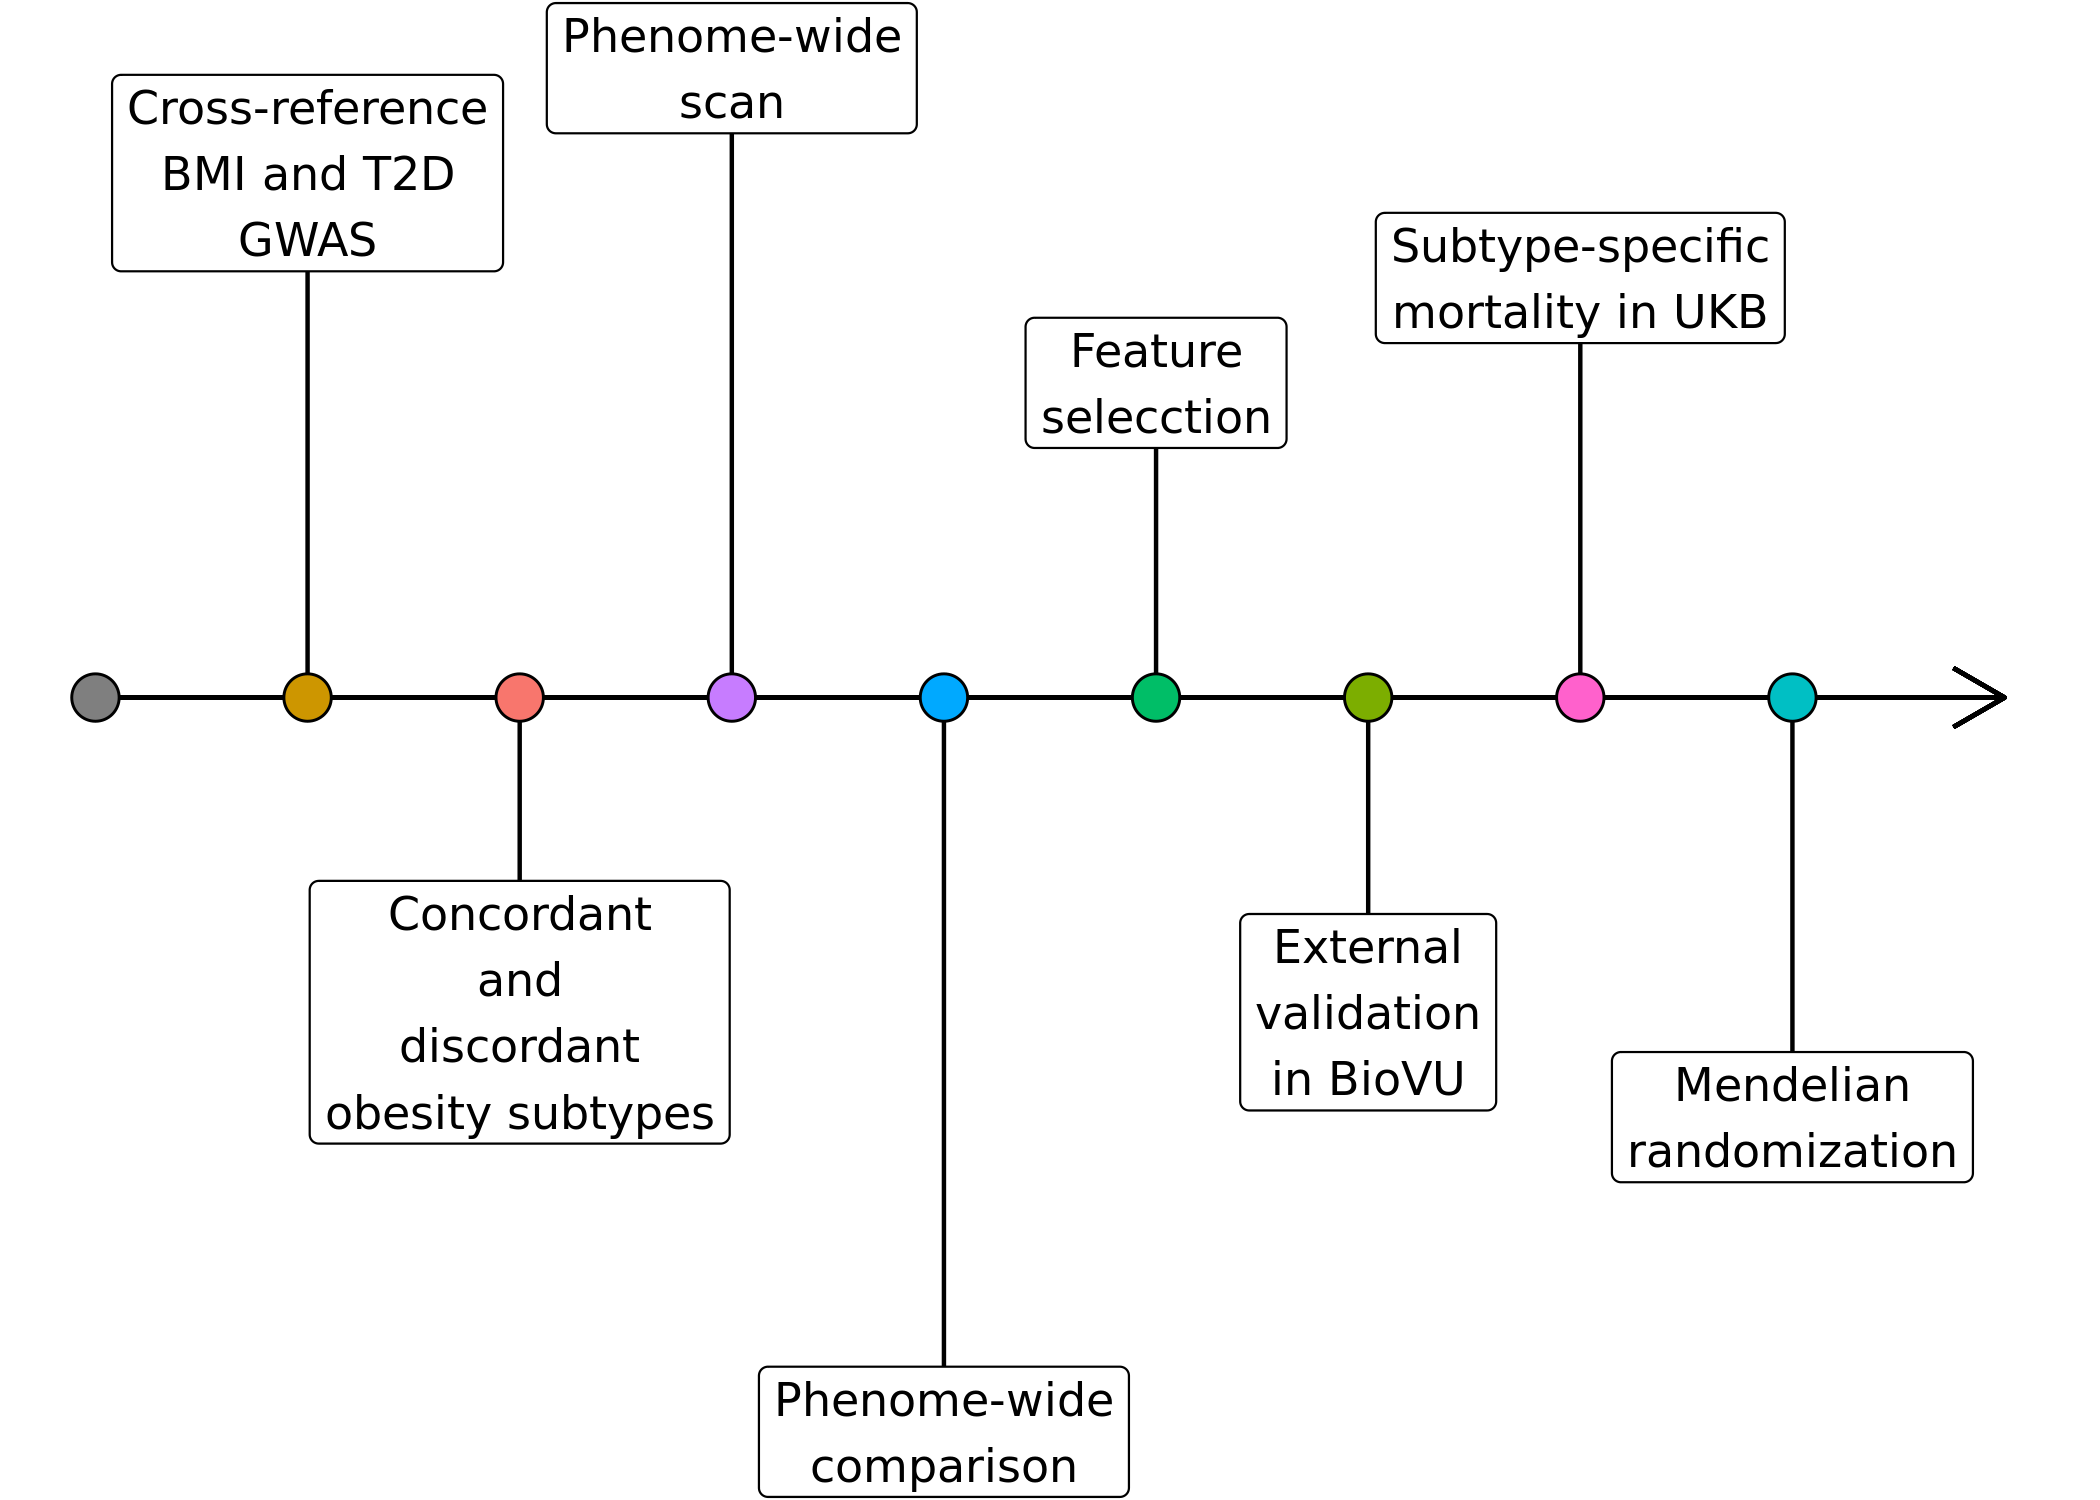
\includegraphics[width=7cm]{./plots/aline_plot.png}
\end{center}
\end{frame}

\begin{frame}[label={sec:org176f804}]{Cross-referencing BMI and T2D GWAS}
BMI from Yengo \emph{et al.} (2018) and T2D from Mahajan \emph{et al} (2018).
\begin{center}
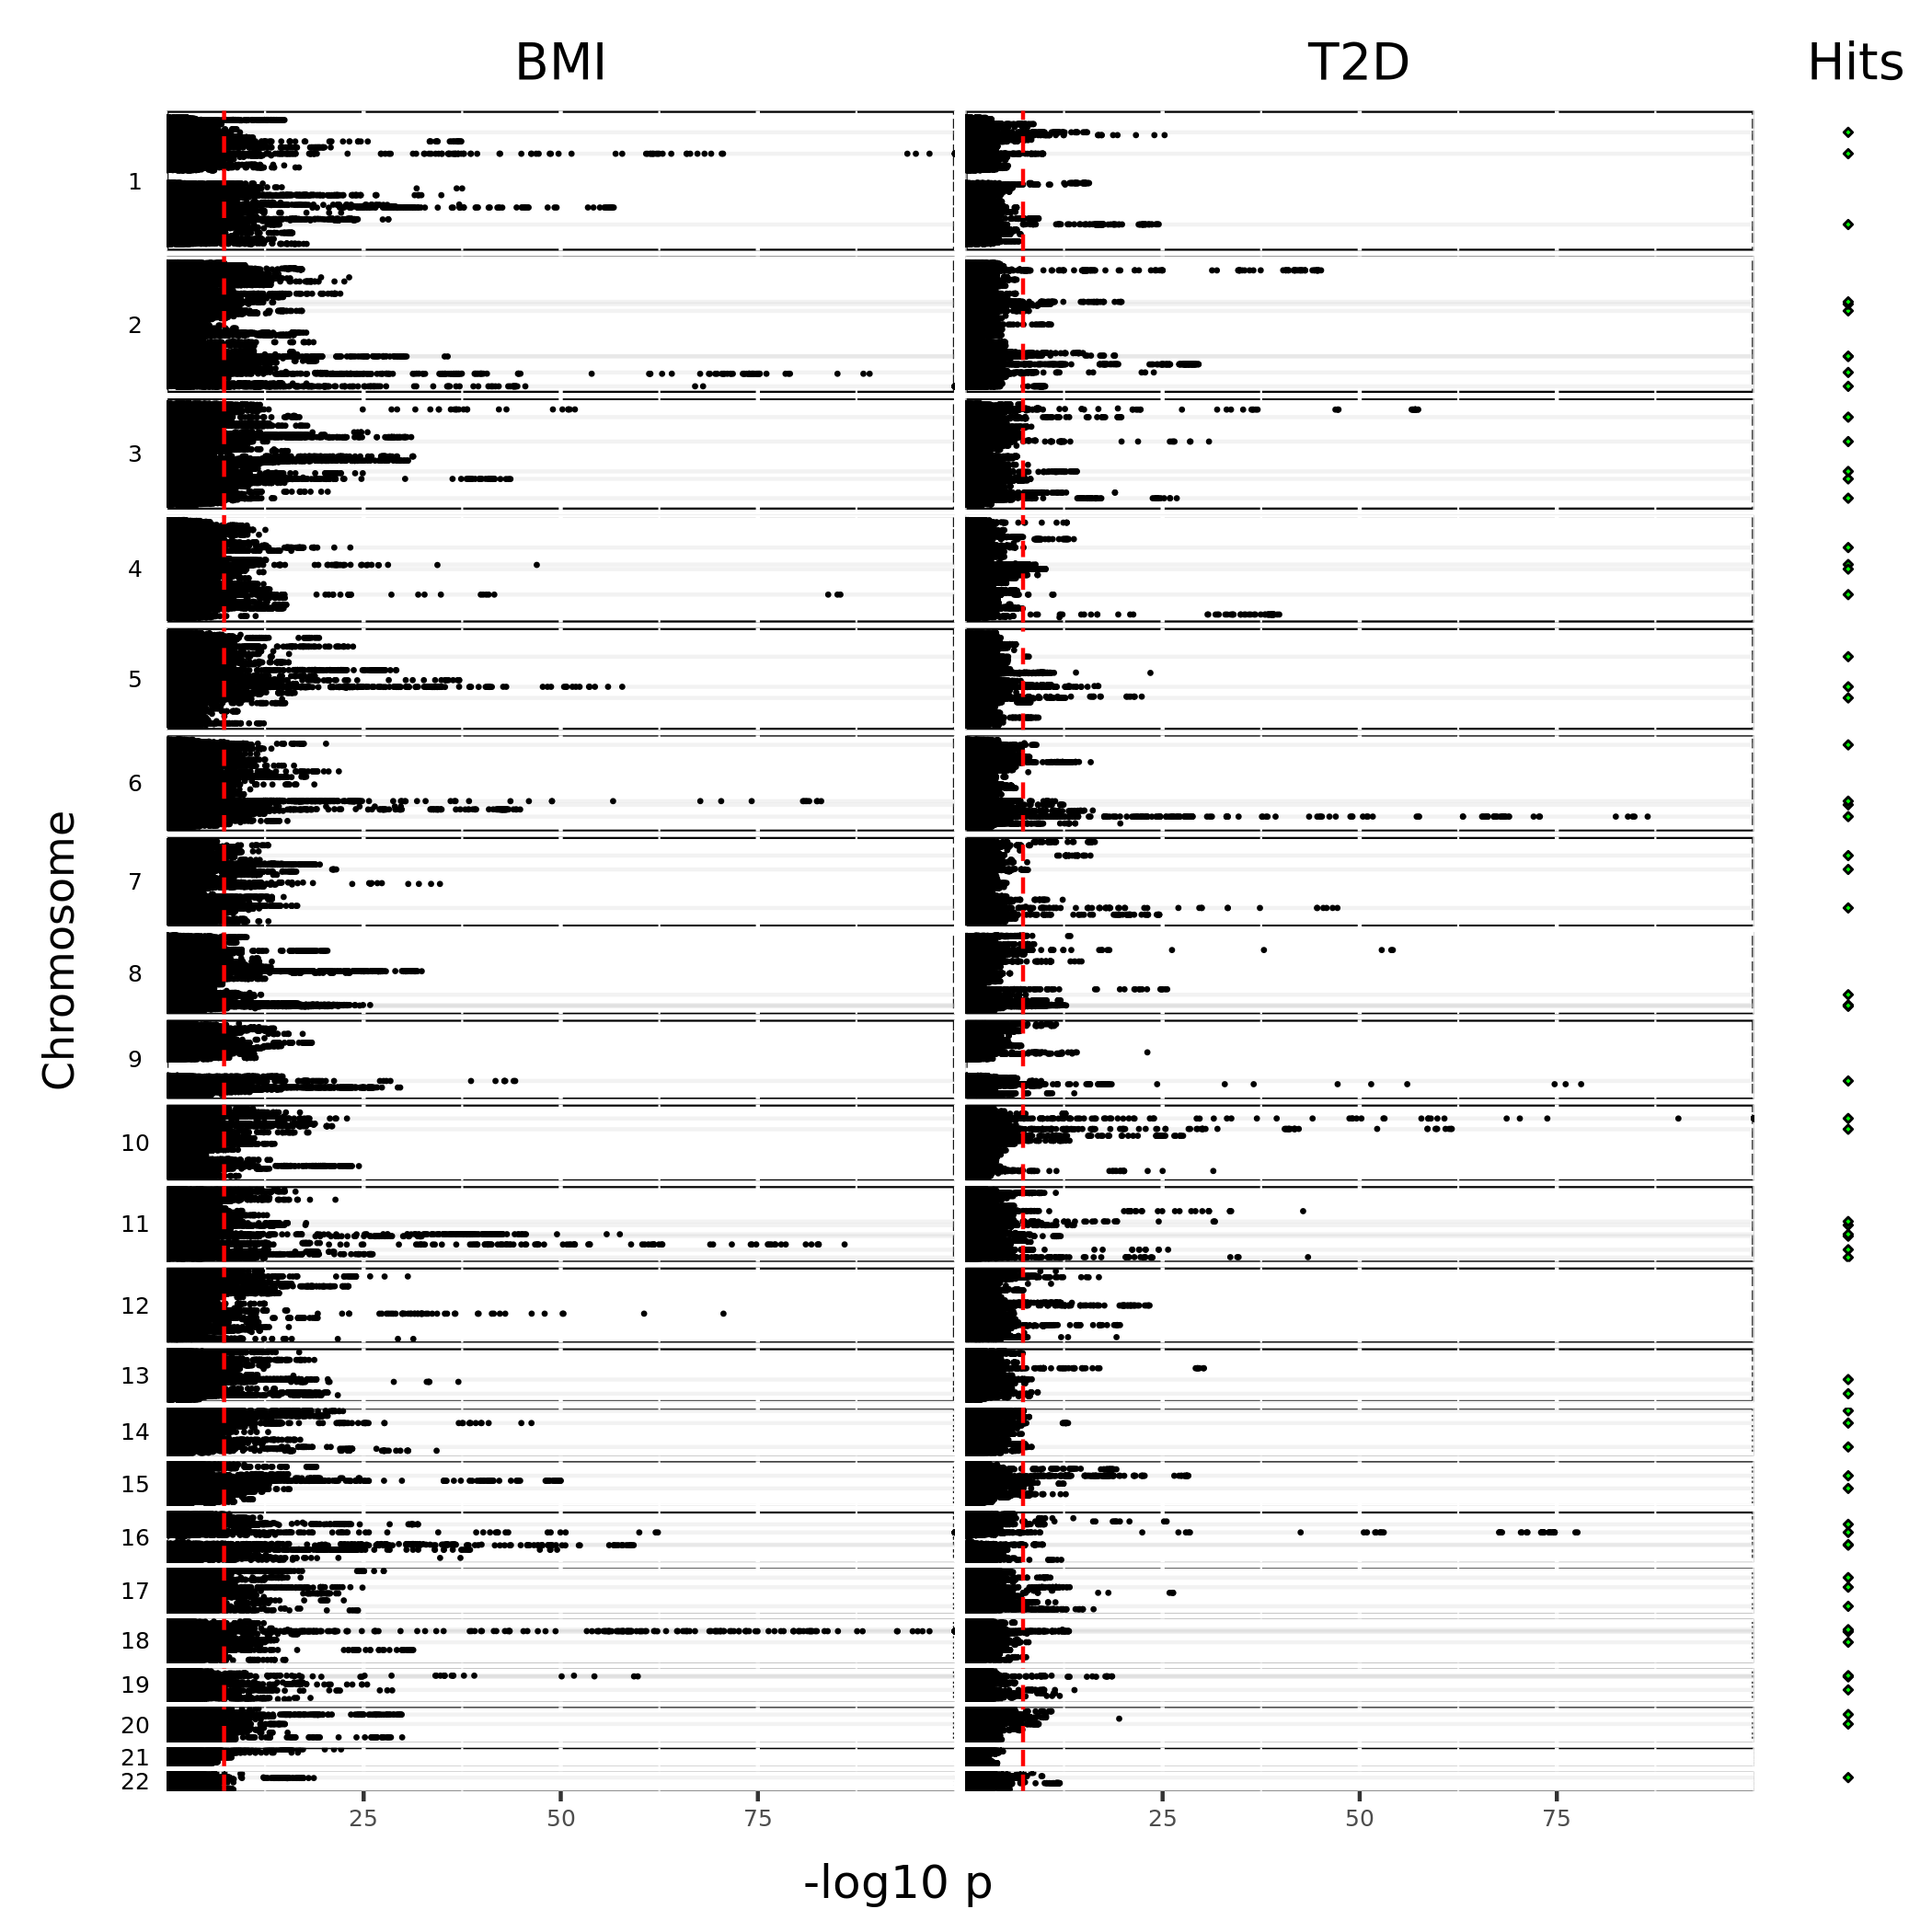
\includegraphics[width=6.5cm]{./plots/gmirror.png}
\end{center}
\end{frame}

\begin{frame}[label={sec:org8513618}]{Assembly of concordant (n = 48) and discordant (n = 19) profiles}
Lead variants aligned to the BMI increasing allele and stratified by their \(\beta\) coefficient for T2D.
\begin{center}
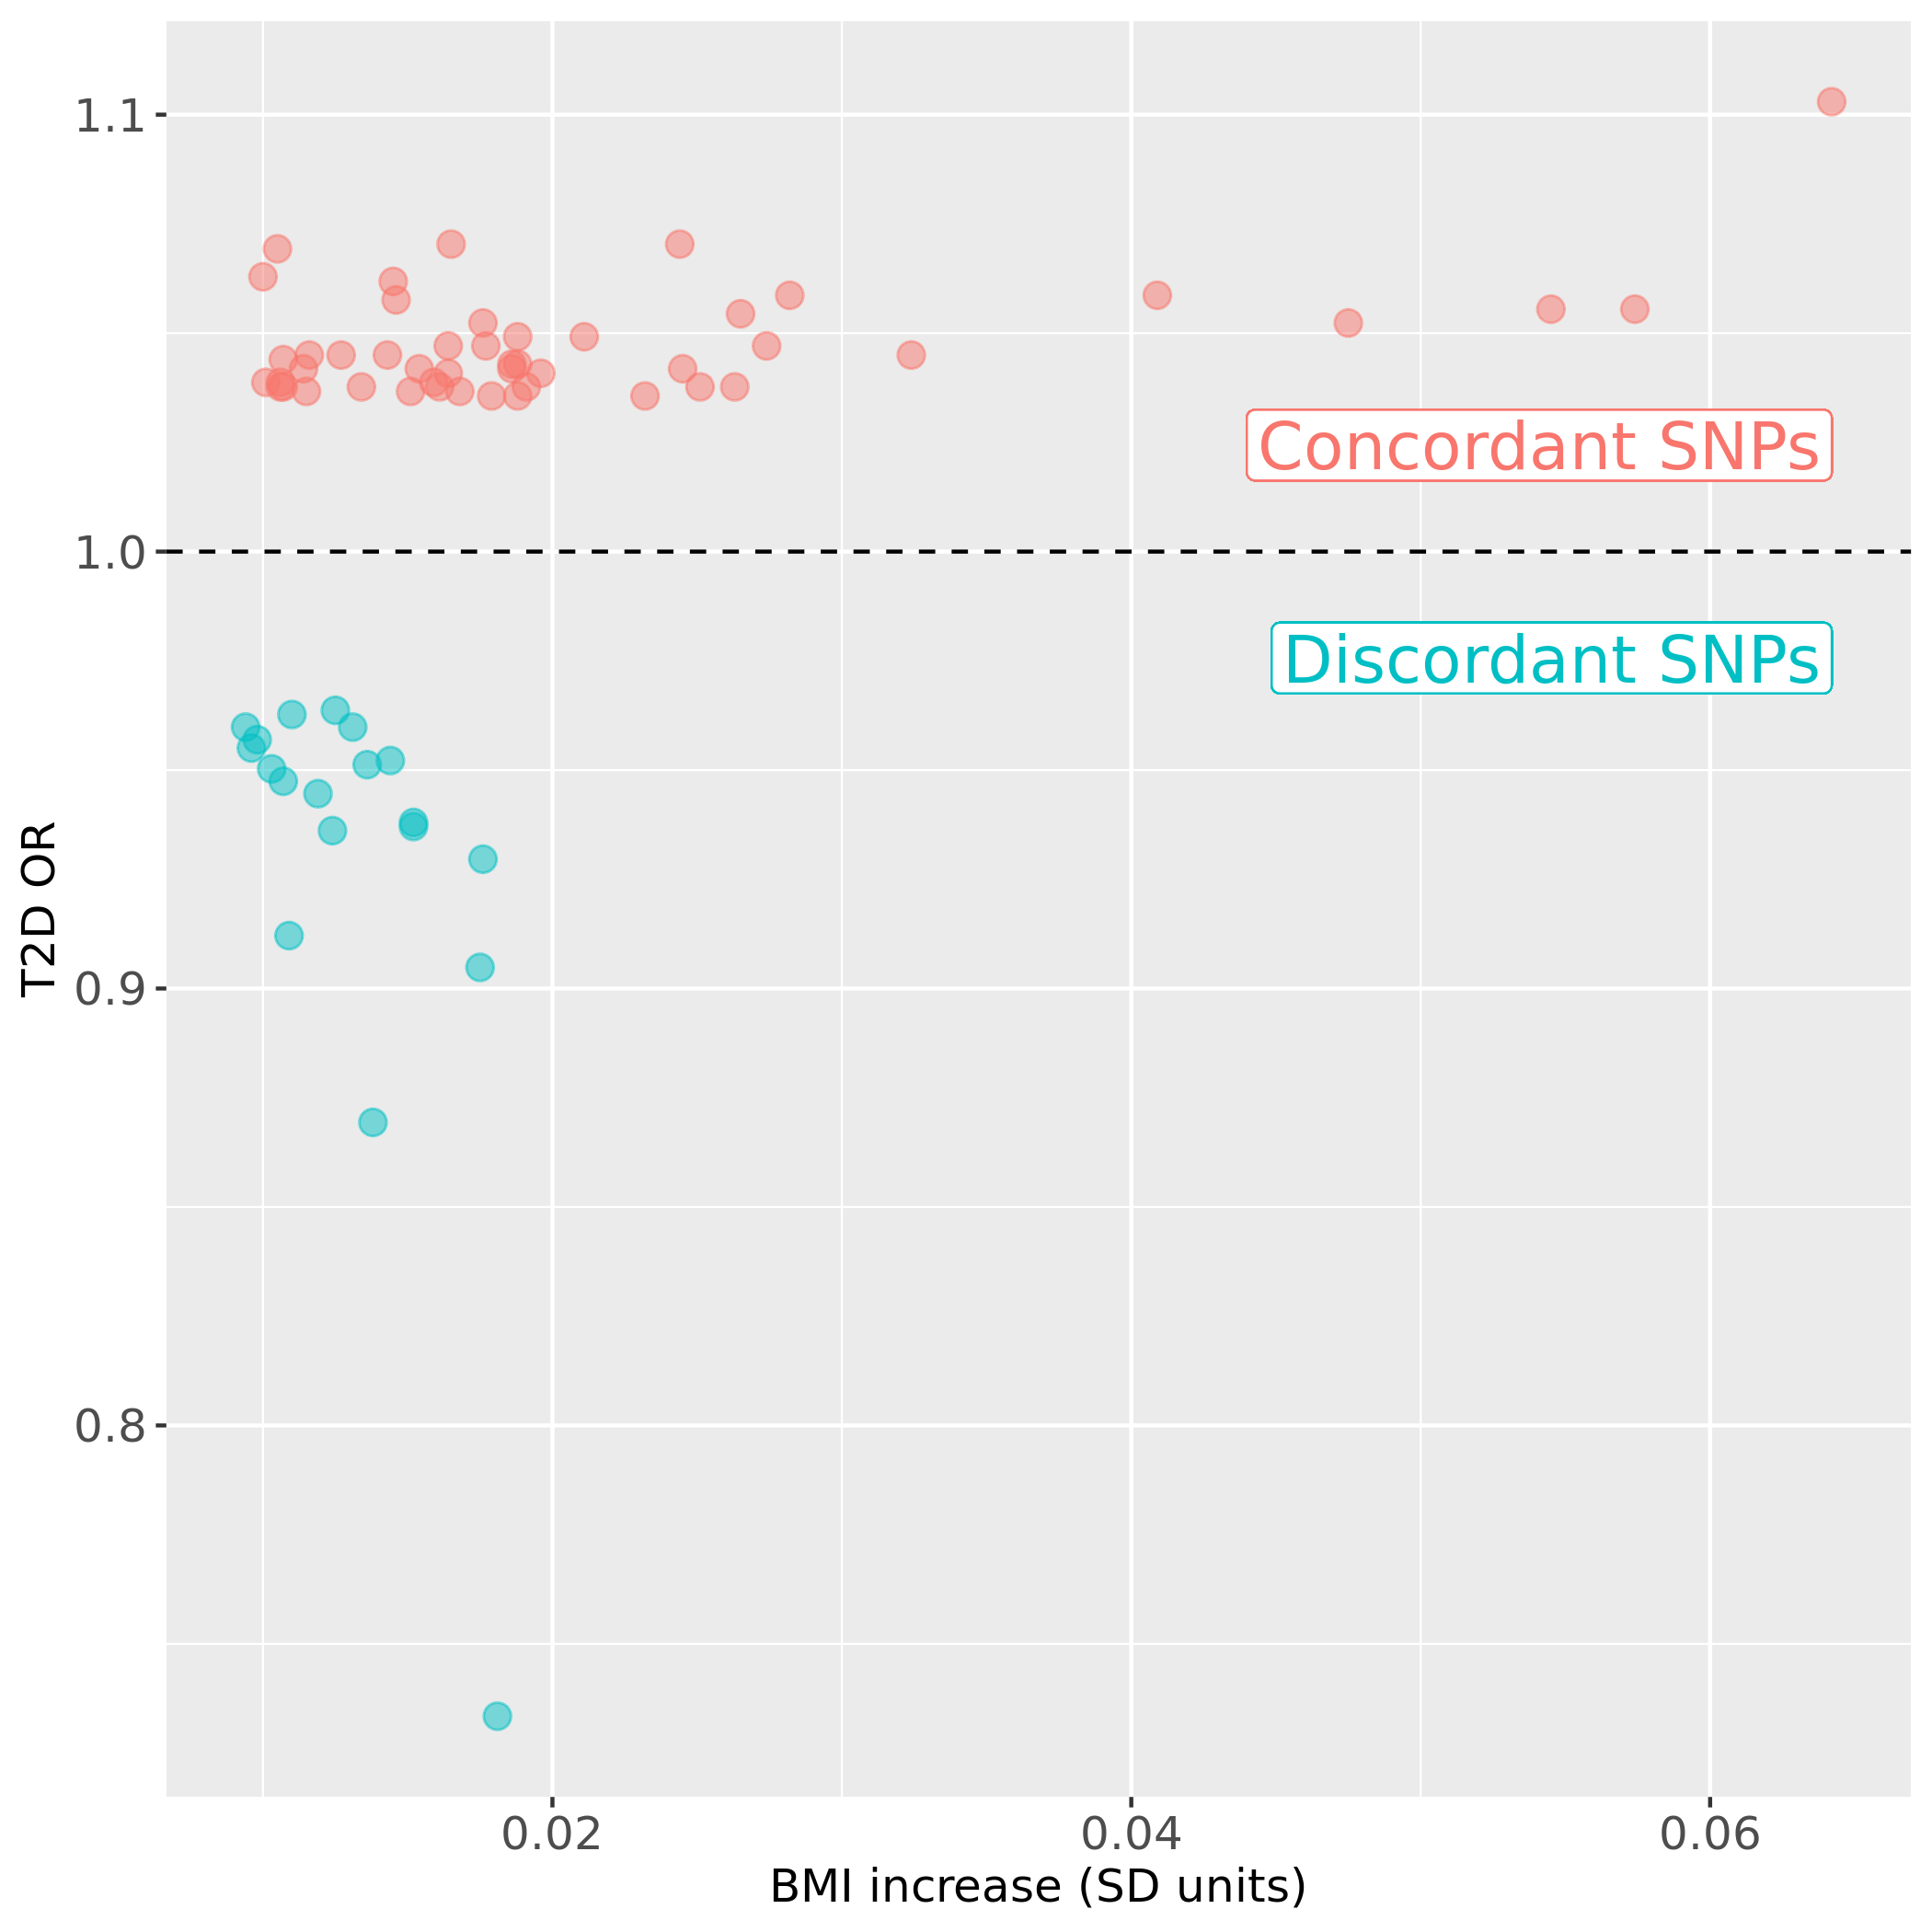
\includegraphics[width=6cm]{./plots/profiles.png}
\end{center}
\end{frame}

\begin{frame}[label={sec:orgdaa4ee1}]{Phenome-wide scan - Data collection}
\begin{itemize}
\item MRC IEU GWAS database
\begin{itemize}
\item Associations of lead SNPs or nearest proxy if missing
\begin{itemize}
\item \emph{r\textsuperscript{2}} < 0.01 over 500kb window in 1000G EUR
\end{itemize}
\item Studies in EUR
\item More than 500 individuals
\item Binary traits: more than 25 minor alleles in smallest group
\end{itemize}
\item \textasciitilde{} 3500 traits
\end{itemize}
\end{frame}

\begin{frame}[label={sec:orgf77fff0}]{Phenome-wide comparison}
\begin{itemize}
\item Two-stage analysis:
\begin{itemize}
\item Univariate comparison
\begin{itemize}
\item Permissive threshold - filter out uninformative traits
\end{itemize}
\item Selection of traits
\begin{itemize}
\item Hierarchical clustering - Random Forest
\end{itemize}
\end{itemize}
\end{itemize}
\end{frame}

\begin{frame}[label={sec:org202d2d0}]{Univariate comparison:}
\begin{itemize}
\item Pooled concordant (\(\beta_C\)) and discordant (\(\beta_D\)) effects for each trait
\begin{itemize}
\item Random effects meta-analysis
\end{itemize}
\item In each trait, are the effects different? (\(|\beta_C - \beta_D|\))
\item Retain traits:
\begin{itemize}
\item Significant difference (FDR 10\%)
\item Any of the two pooled estimates significant (FDR 10\%)
\end{itemize}
\end{itemize}
\end{frame}

\begin{frame}[label={sec:orgd596f81}]{Results of univariate comparison (n = 195)}
\begin{itemize}
\item Significant differences (FDR 10\%) between pooled estimates
\end{itemize}
\begin{center}
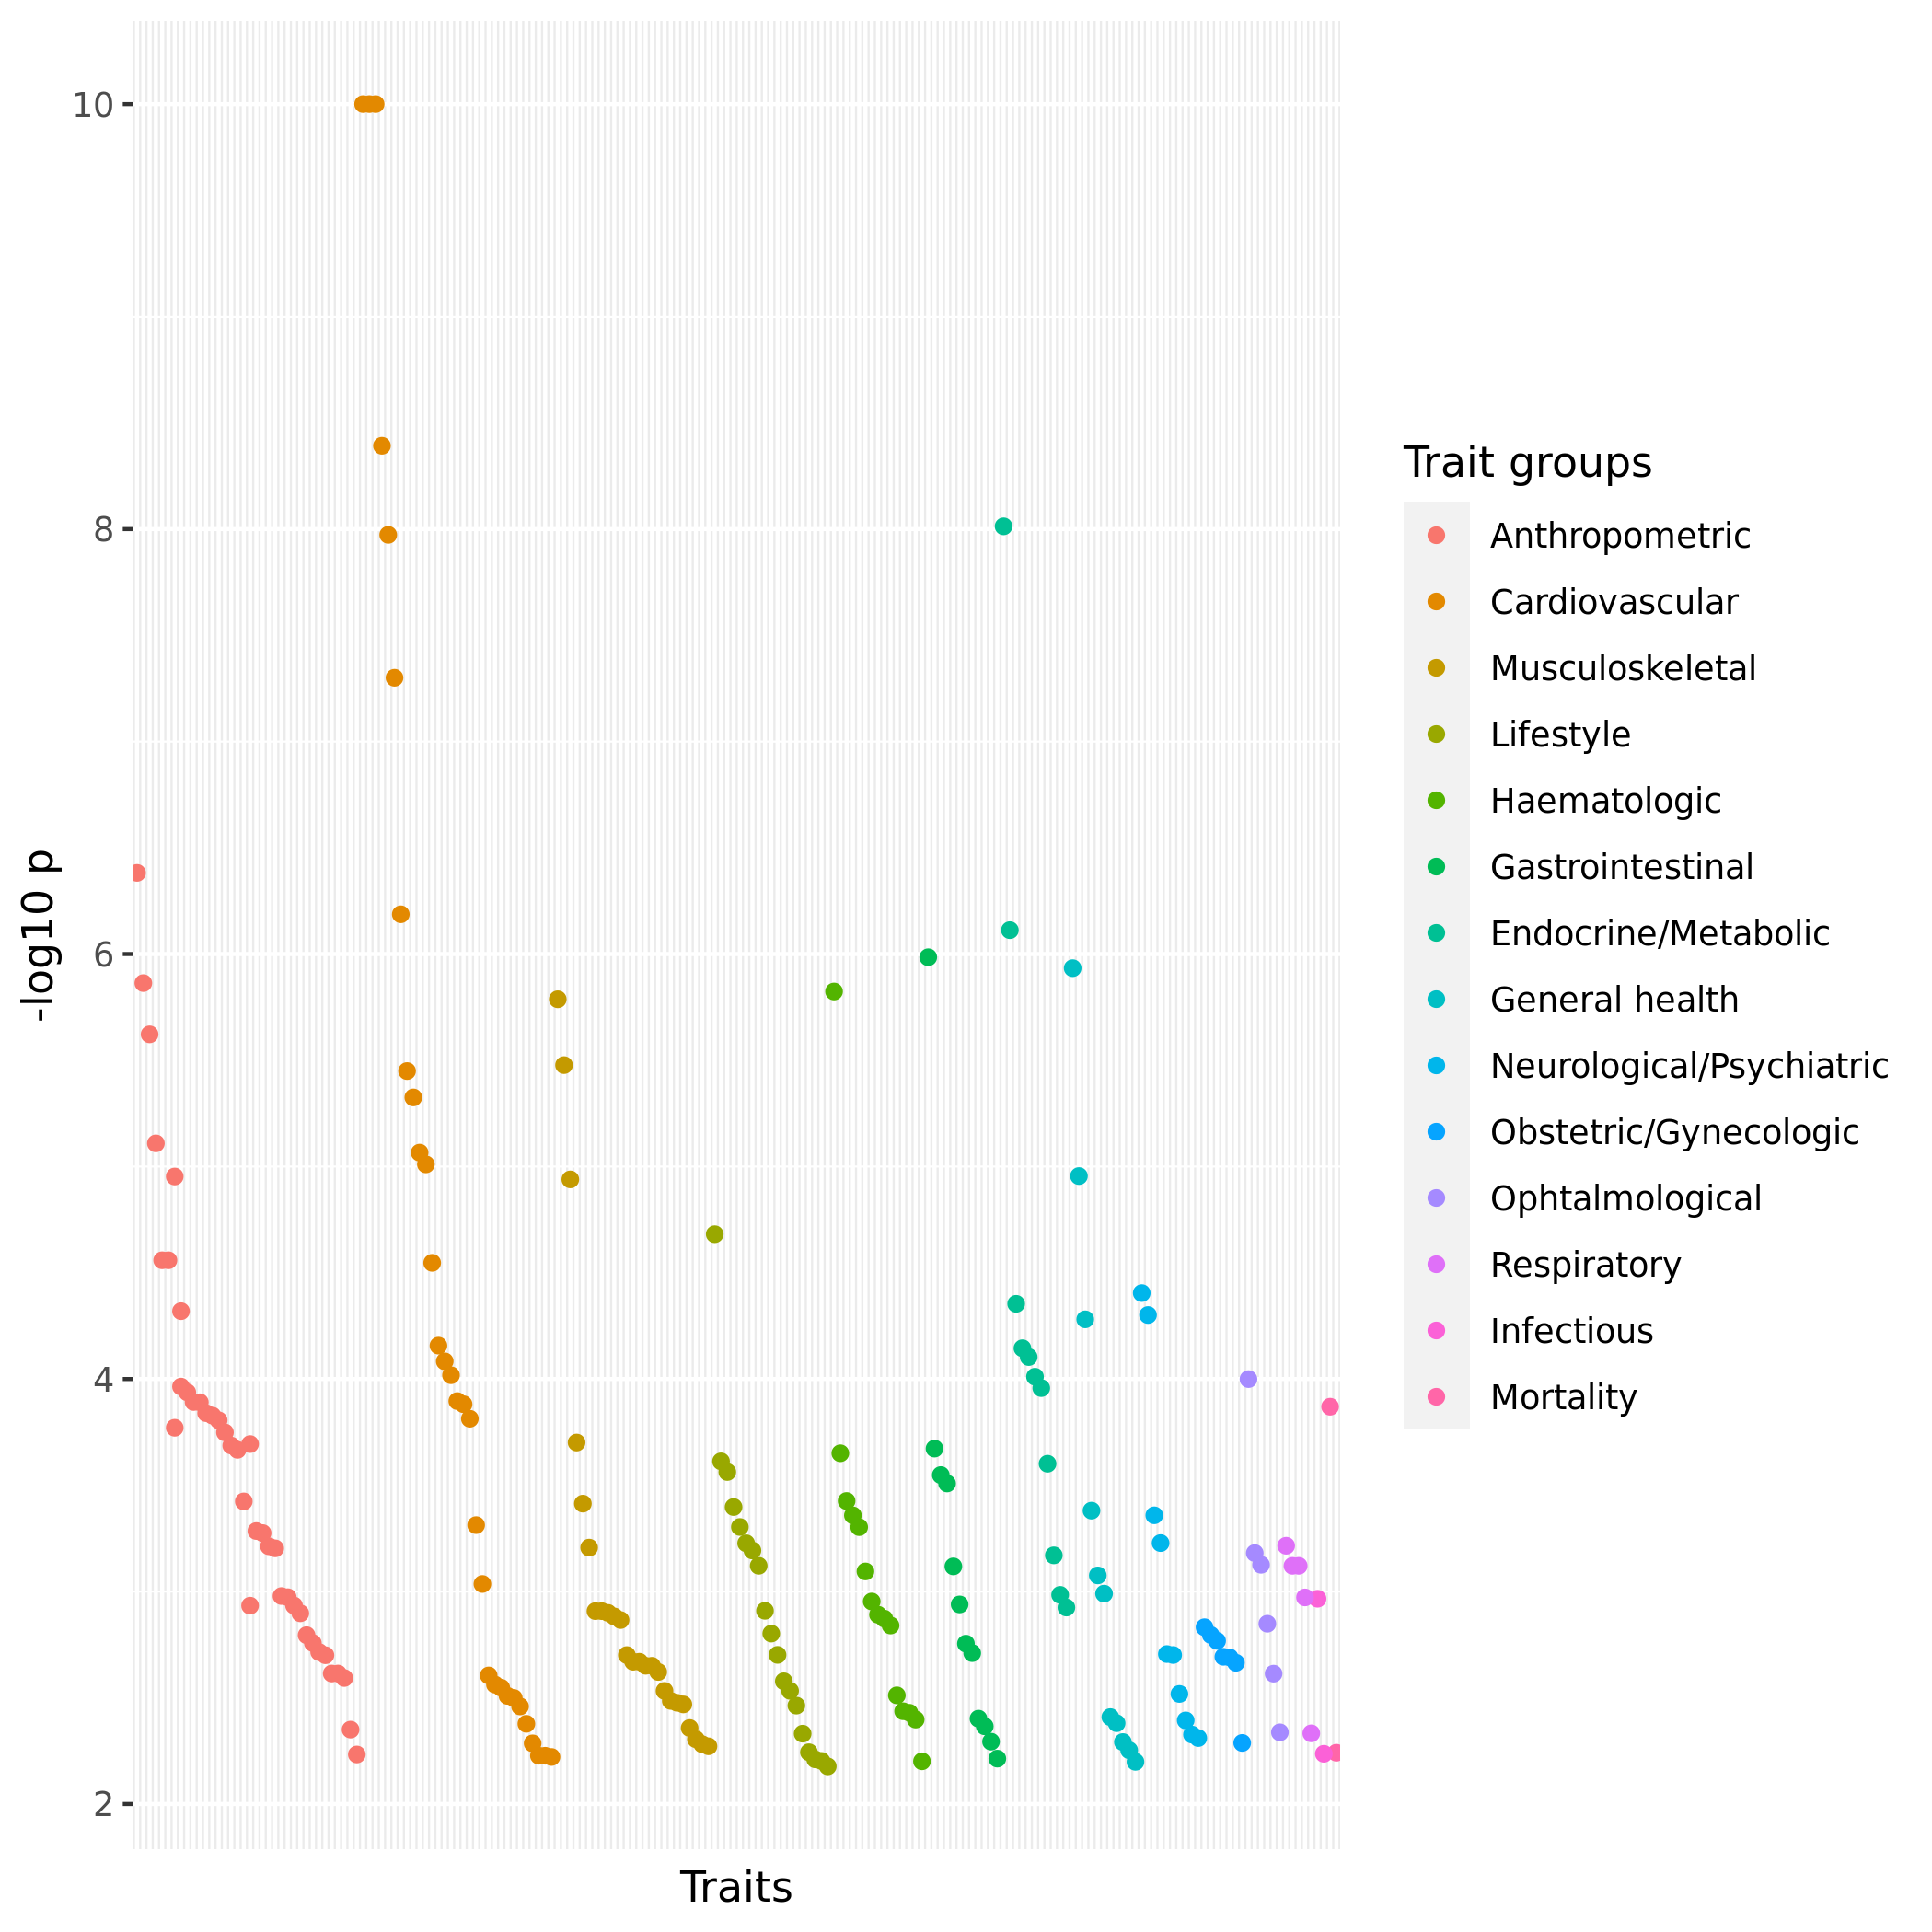
\includegraphics[width=7cm]{./plots/phewas_res.png}
\end{center}
\end{frame}

\begin{frame}[label={sec:org0bf5a98}]{SNP-Trait matrix}
\begin{itemize}
\item For each SNP in each trait:
\end{itemize}
\begin{align*}
Z = \frac{\beta}{SE_{\beta}}
\end{align*}

\begin{center}
\begin{tabular}{llllll}
SNP & \alert{Discordant} & Trait\textsubscript{1} & Trait\textsubscript{2} & \ldots{} & Trait\textsubscript{p}\\
\hline
SNP1 & Yes & \(Z_{11}\) & \(Z_{12}\) & \ldots{} & \(Z_{1p}\)\\
SNP2 & No & \(Z_{21}\) & \(Z_{22}\) & \ldots{} & \(Z_{2p}\)\\
SNP3 & Yes & \(Z_{31}\) & \(Z_{32}\) & \ldots{} & \(Z_{3p}\)\\
\ldots{} & \ldots{} & \ldots{} & \ldots{} & \ldots{} & \ldots{}\\
SNPn & Yes & \(Z_{n1}\) & \(Z_{n2}\) & \ldots{} & \(Z_{np}\)\\
\end{tabular}
\end{center}

\begin{itemize}
\item High dimensionality
\item Multicolinearity
\item COVVSURF (Chavent \emph{et al.} 2019)
\begin{itemize}
\item Hierarchical clustering - Random forest
\end{itemize}
\end{itemize}
\end{frame}

\begin{frame}[label={sec:orgbbbedc0}]{Hierarchical clustering}
\begin{itemize}
\item At each ascending step:
\begin{enumerate}
\item Starting point: each trait is a cluster
\item Compute PCA between each pair
\begin{itemize}
\item Obtain PC1 - Captures most variation of members
\end{itemize}
\item Group most similar pair into a cluster
\begin{itemize}
\item \(\sum_{j=1}^j r^2_{x_j, PC_1}\)
\end{itemize}
\end{enumerate}
\item Iterate until all traits are clustered together
\end{itemize}
\end{frame}

\begin{frame}[label={sec:org6739f58}]{PCA as measure of similarity}
\begin{itemize}
\item At every possible partition (\emph{i.e.} number of clusters \emph{k}):
\end{itemize}
\begin{center}
Each cluster (\(C_1, C_2, ..., C_k\))\\
\(\Downarrow\)\\
can be summarized by\\
\(\Downarrow\)\\
The correspoding PC1s (\(PC1_1, PC1_2, ..., PC1_k\))
\end{center}
\end{frame}

\begin{frame}[label={sec:orgbf3fccf}]{Recap Random Forest (RF)}
\begin{itemize}
\item Robust non-parametric classifier
\item Multiple decision trees:
\begin{itemize}
\item Grown using a random subset of data (in-bag)
\item At each split, selects the trait that minimizes variance in child nodes
\item Estimation of error rate / accuracy
\begin{itemize}
\item Average out-of-bag (OOB) error of trees
\end{itemize}
\end{itemize}
\end{itemize}
\end{frame}

\begin{frame}[label={sec:org99c06ca}]{Optimizing partition using RF}
\begin{itemize}
\item At each \emph{k}, take \(PC1_1, PC1_2, ..., PC1_k\) as predictors for random forest
\item Compute error rate
\item Select \emph{k} where the model has the lowest error rate
\end{itemize}
\begin{center}
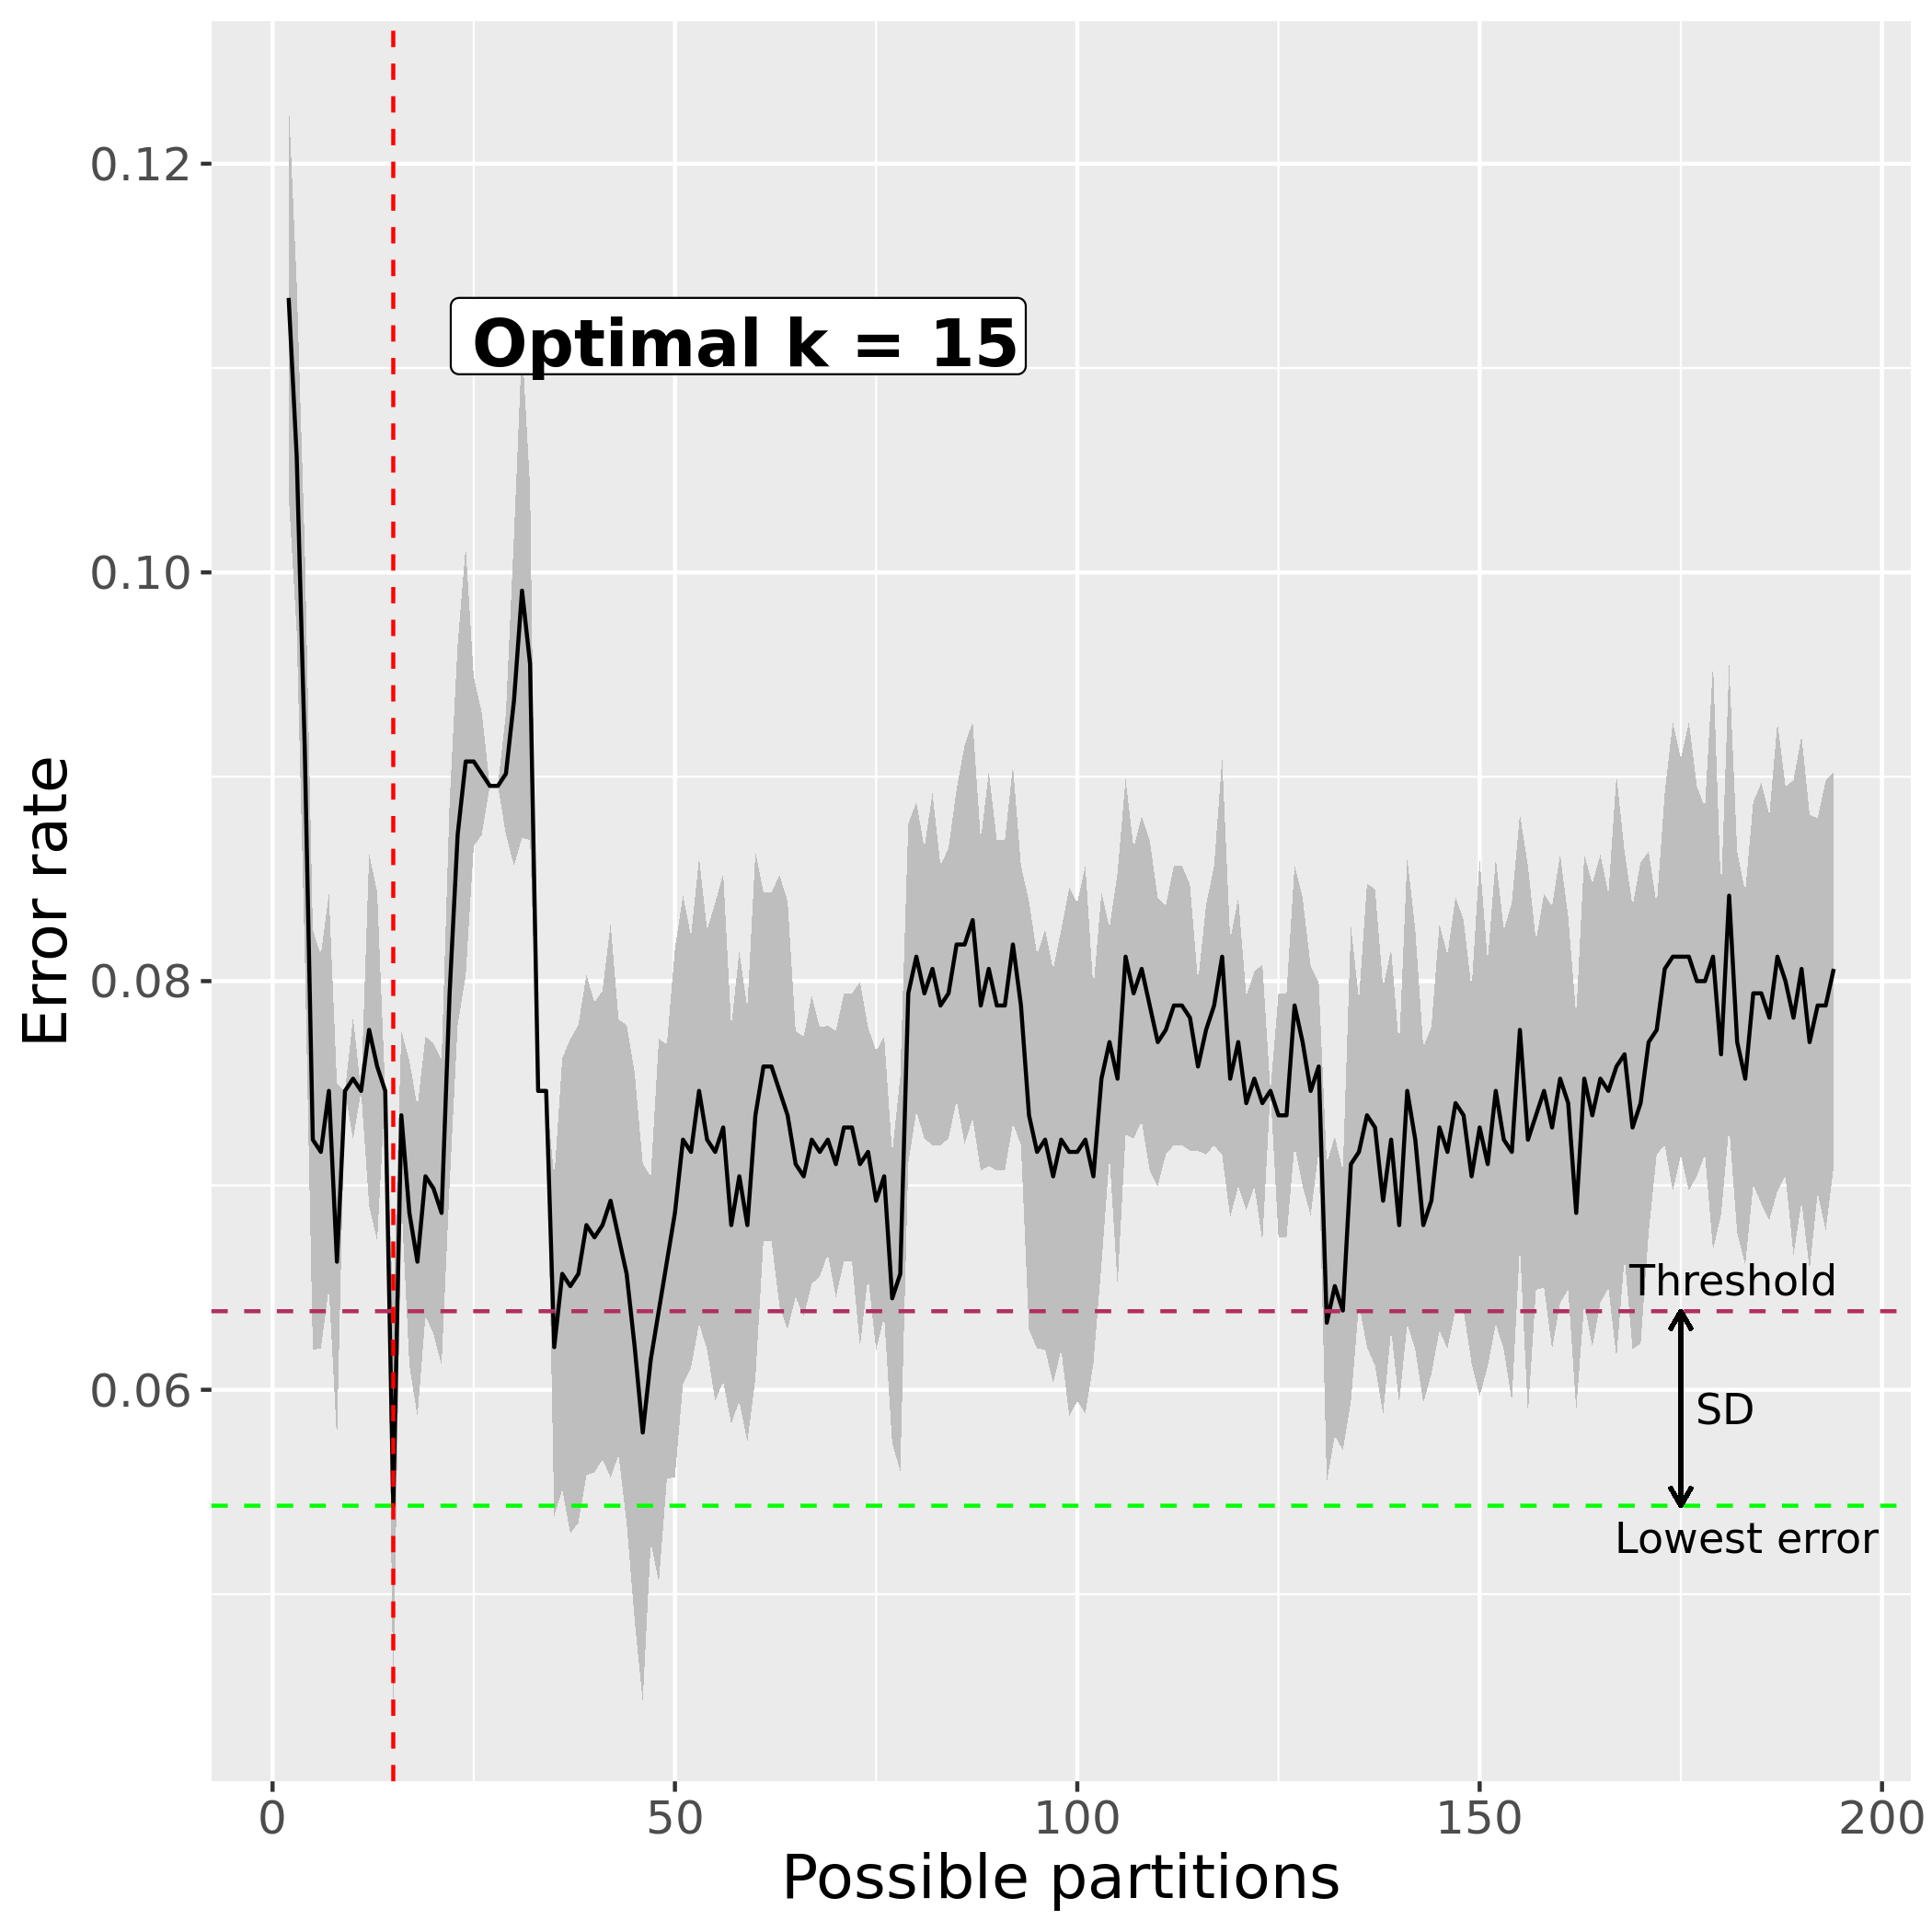
\includegraphics[width=6cm]{./plots/kopt_phen.png}
\end{center}
\end{frame}

\begin{frame}[label={sec:orgf6385cc}]{Clusters of traits}
\begin{center}
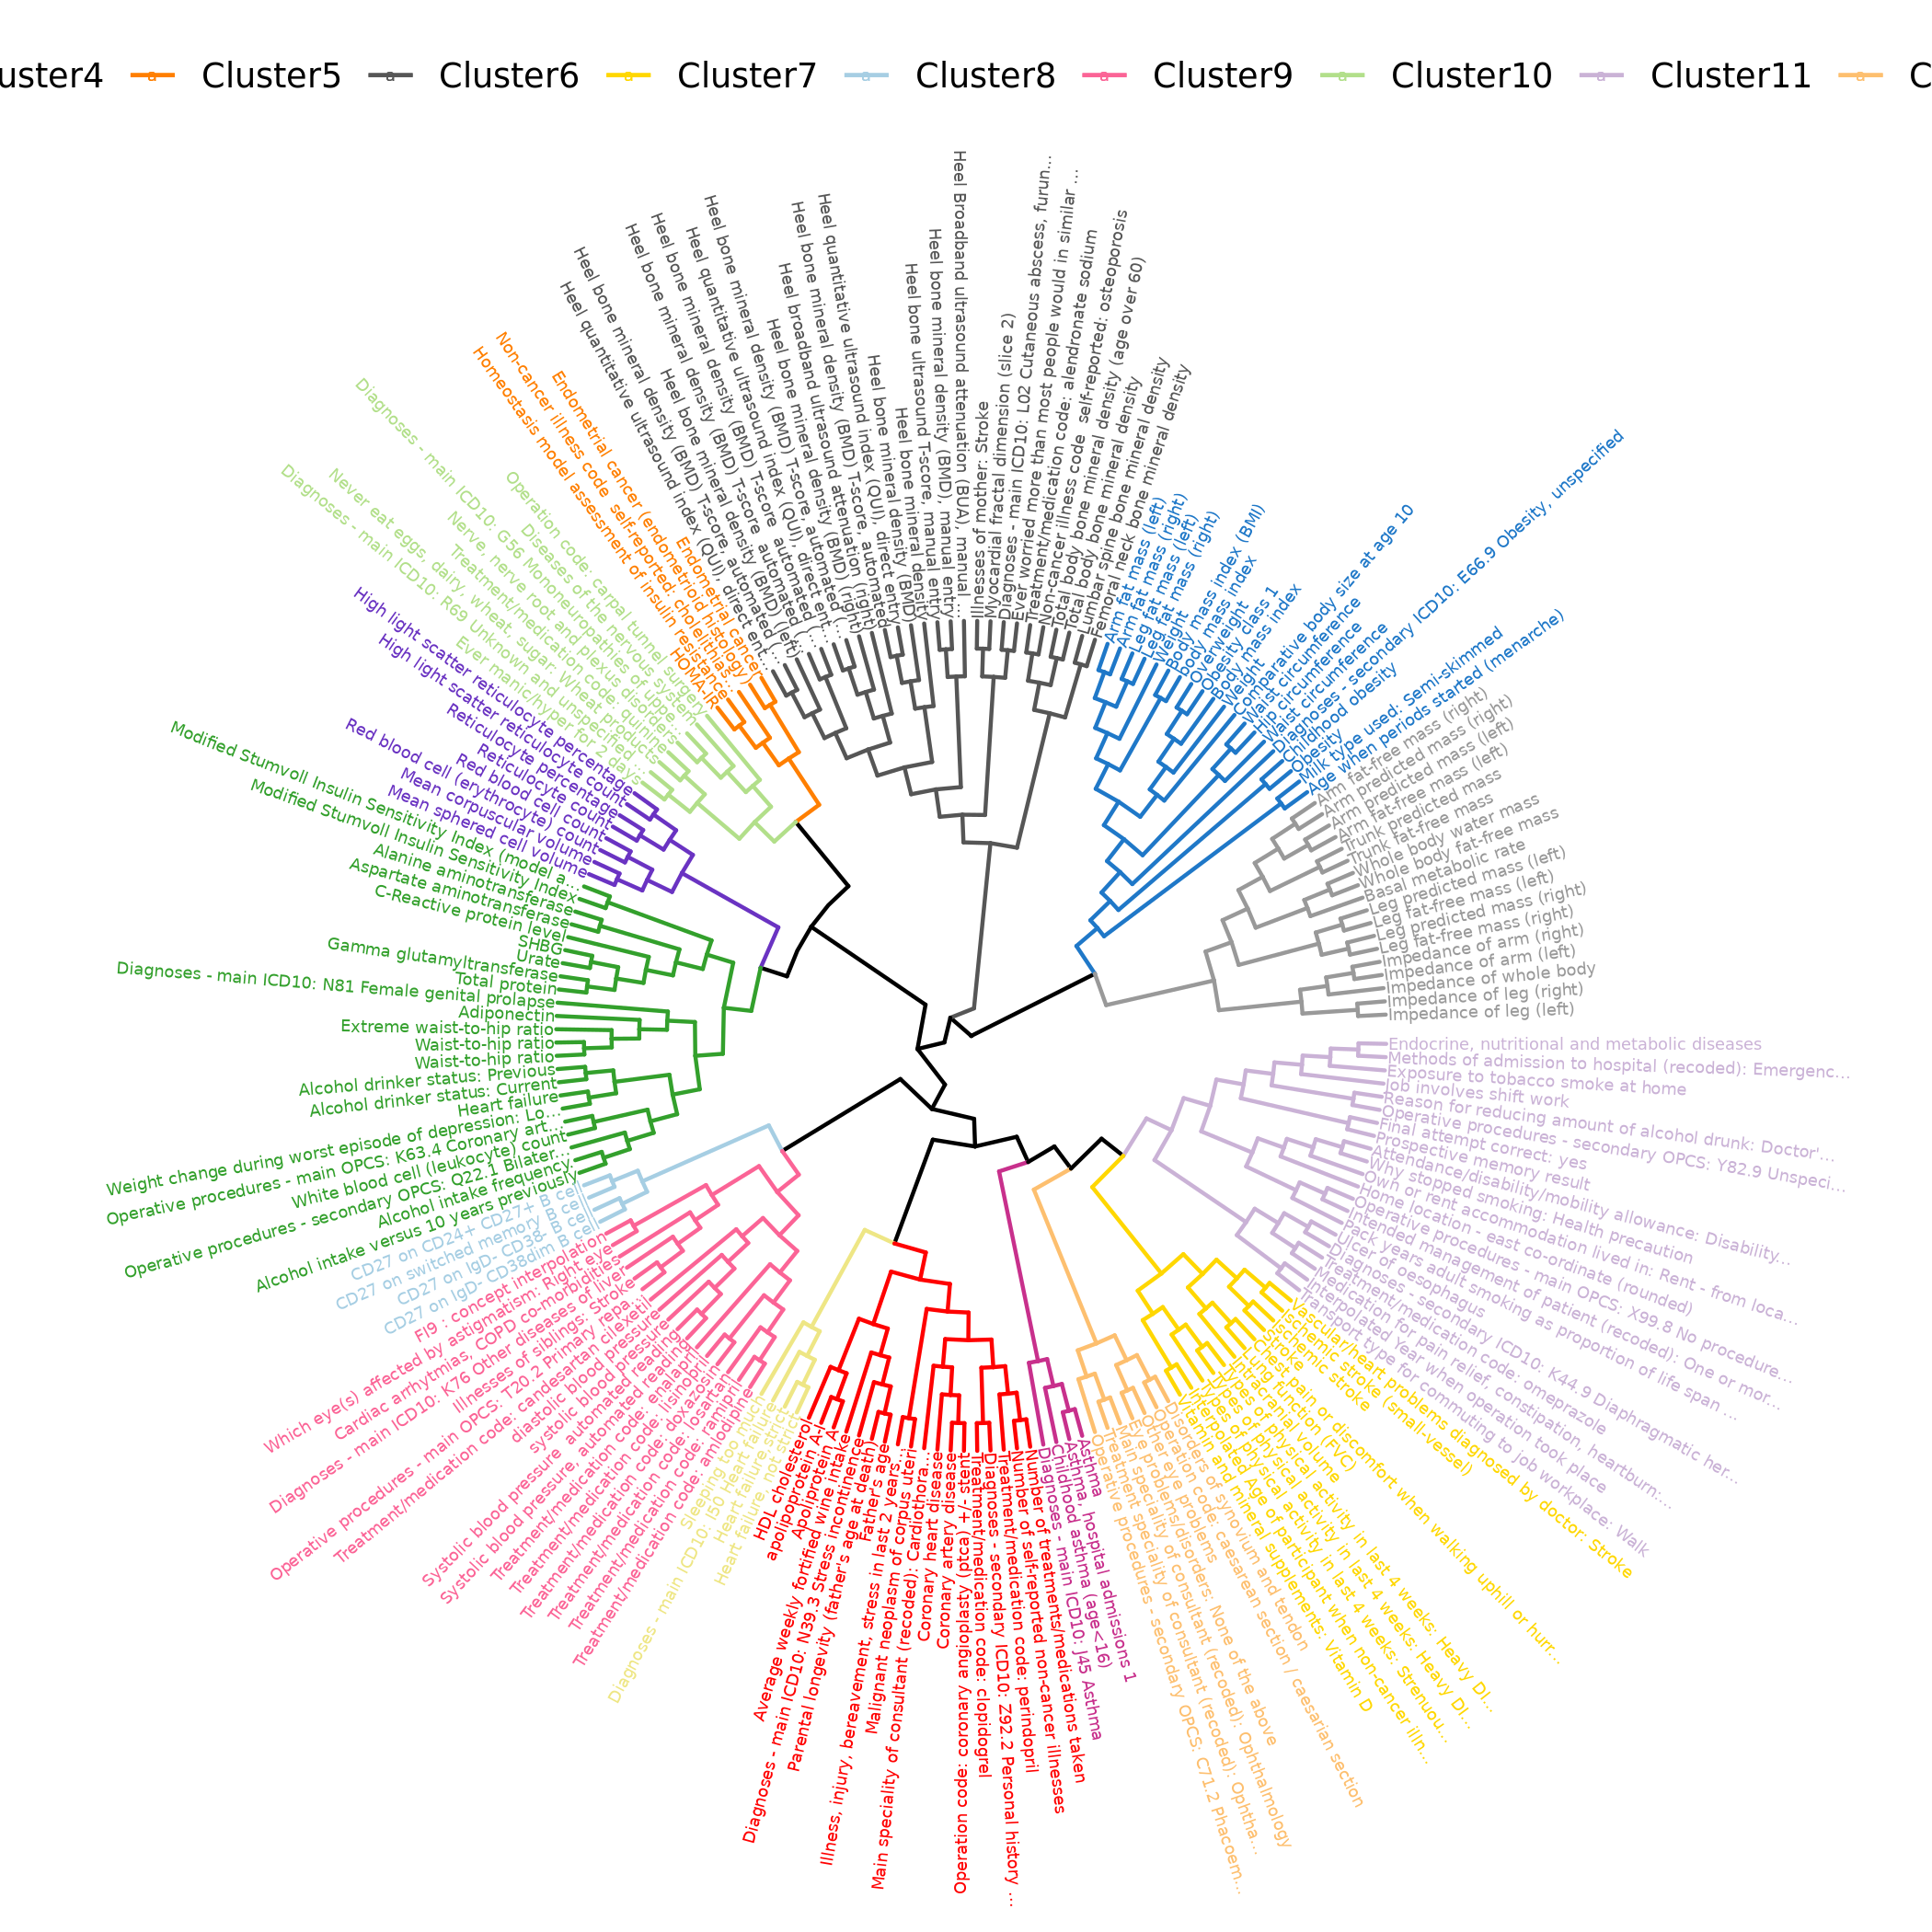
\includegraphics[width=7cm]{./plots/dend_phen.png}
\end{center}
\end{frame}

\begin{frame}[label={sec:orgaf69e43}]{Importance score}
\begin{itemize}
\item \(Imp_{v_p}\) = Average OOB error rate increase of trees when \(v_p\)is absent
\item Nested models >> Final model - minimum OOB error rate.
\end{itemize}
\begin{center}
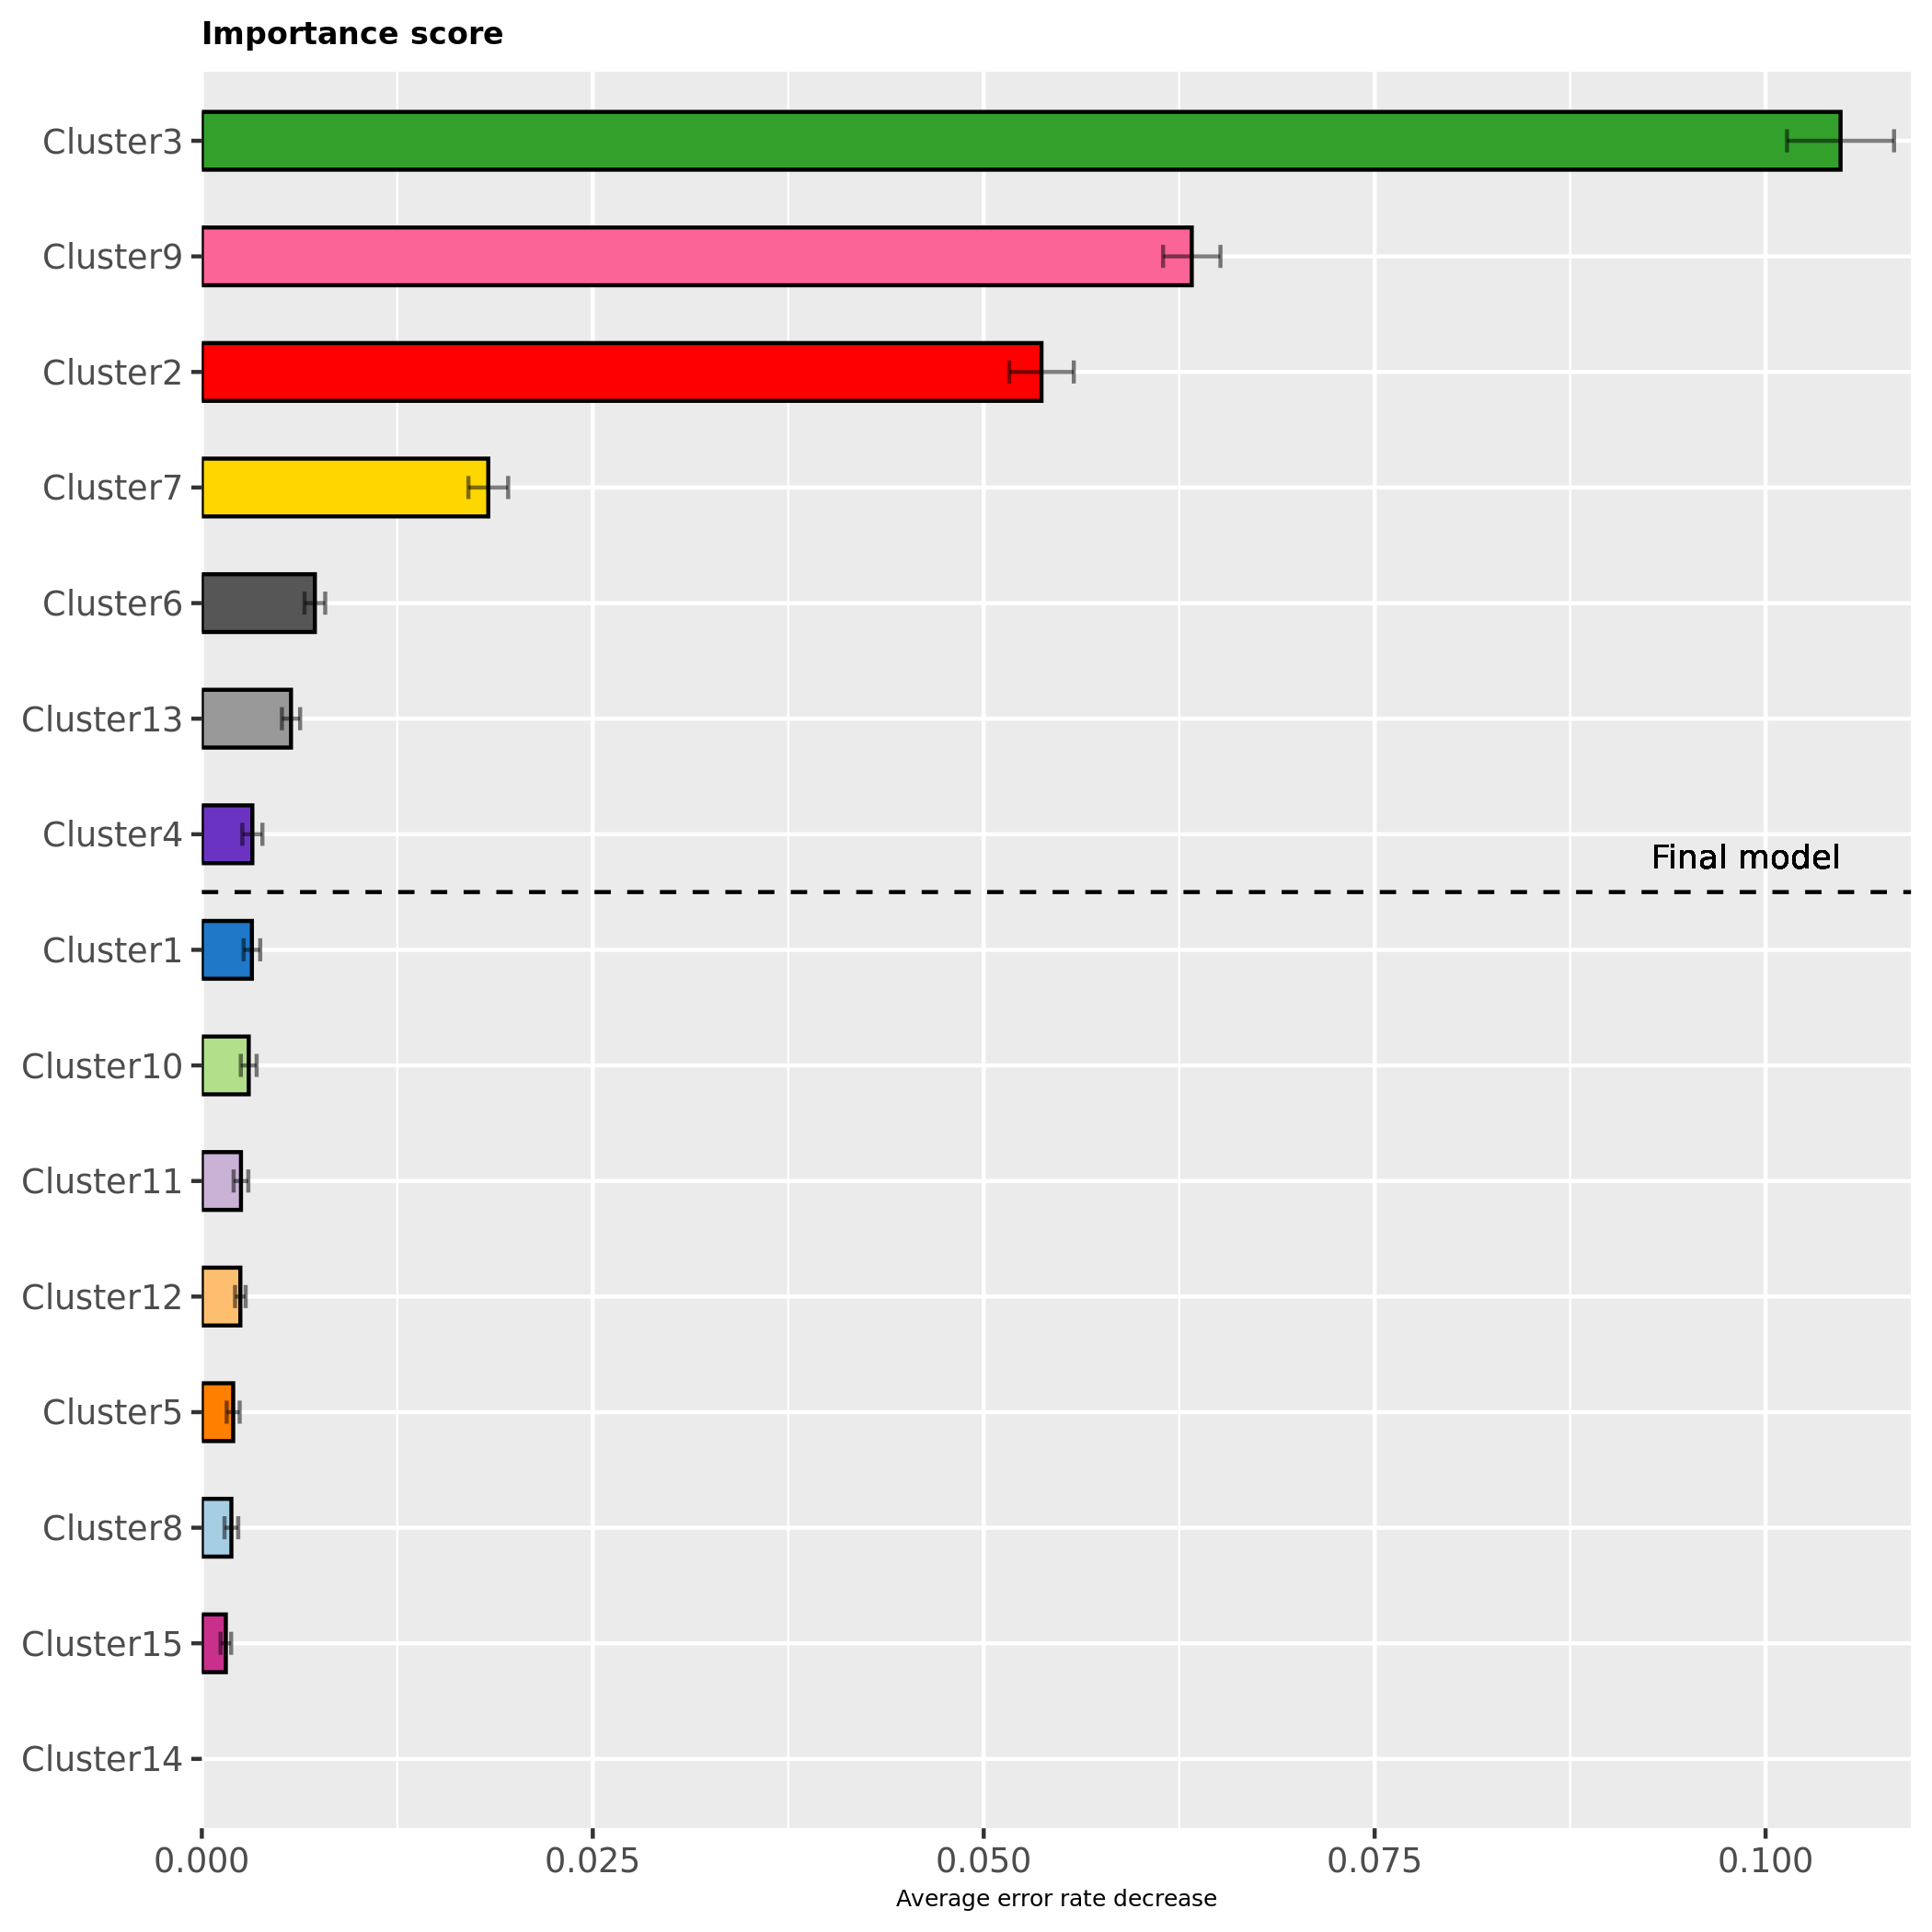
\includegraphics[width=5cm]{./plots/clusimp_phen.png}
\end{center}
\end{frame}

\begin{frame}[label={sec:orgdfdfd74}]{Final model}
\begin{itemize}
\item The relevance of a cluster is given by the importance score
\item Within each cluster, the relevance of a trait is given by its squared loading to the PC1 of the cluster
\end{itemize}
\begin{center}
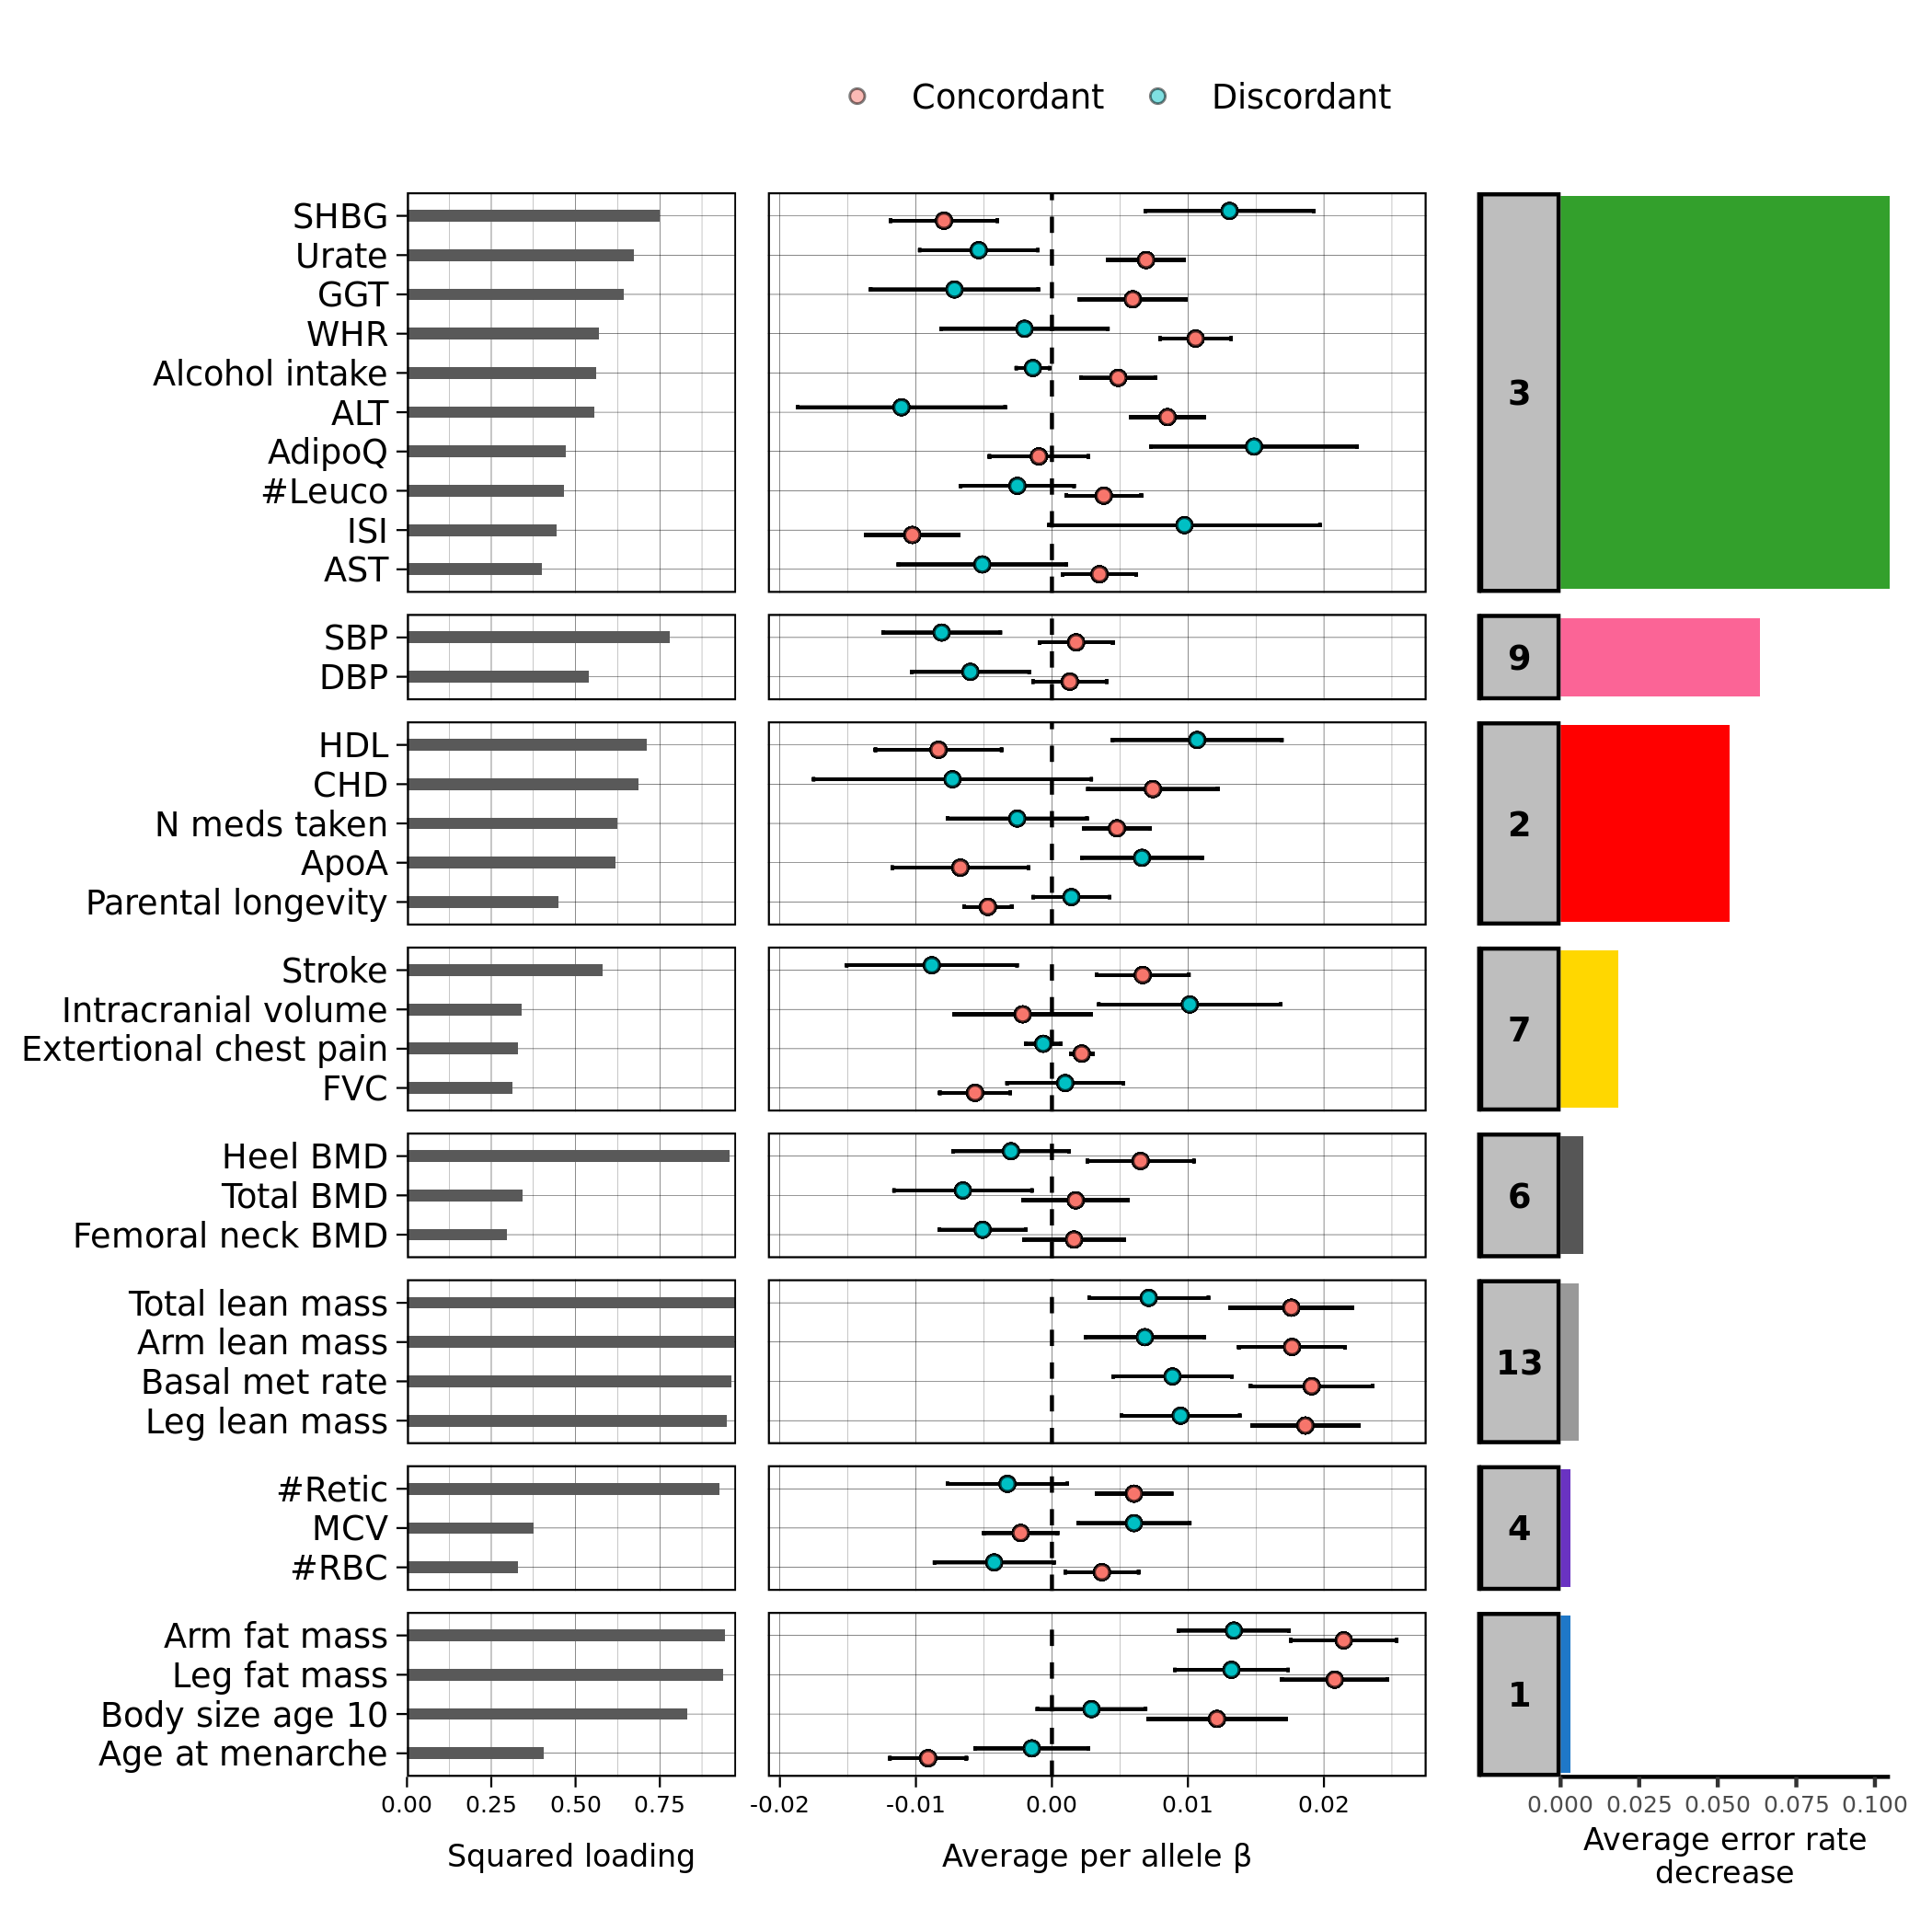
\includegraphics[width=6cm]{./plots/clus_str_phen.png}
\end{center}
\end{frame}

\begin{frame}[label={sec:orgbfb703d}]{The 3 main variables}
\begin{center}
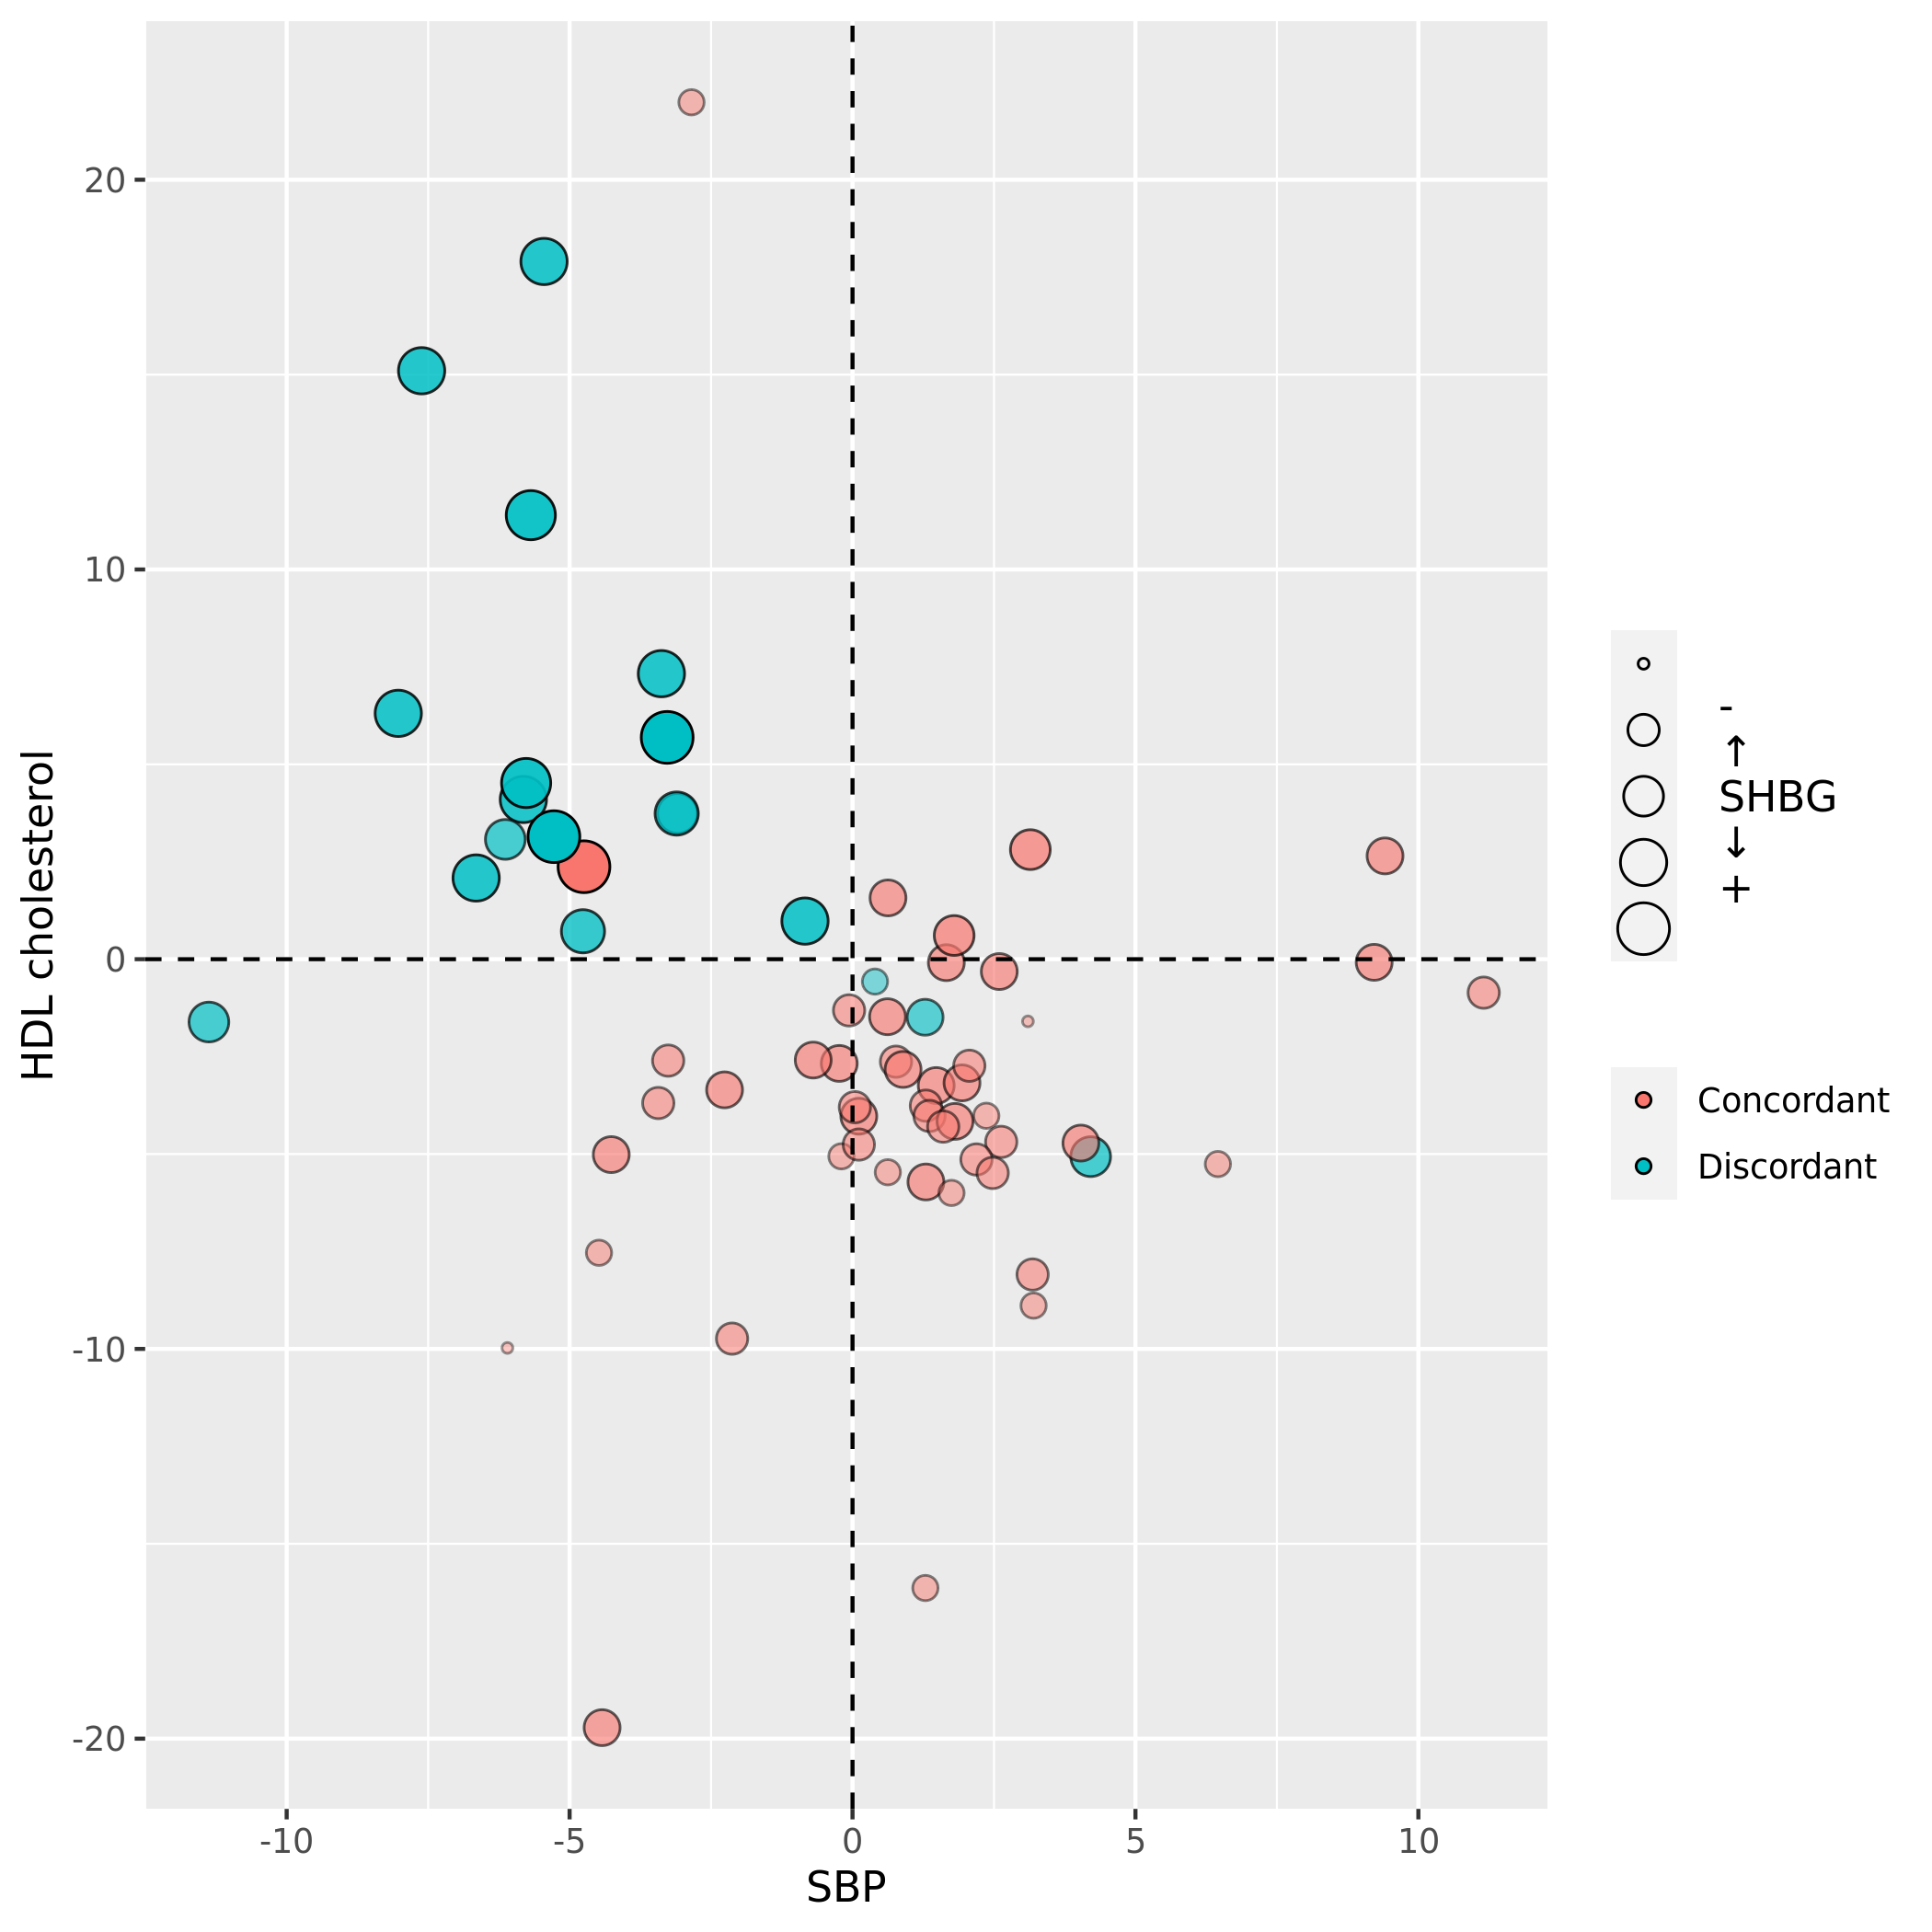
\includegraphics[width=6cm]{./plots/mainvars_phen.png}
\end{center}
\end{frame}

\begin{frame}[label={sec:org32a3154}]{RF Proximity matrix}
\begin{itemize}
\item RF proximity: N times two observations occupy the same terminal node
\item SNP x SNP proximity matrix
\item First two dimensions:
\end{itemize}
\begin{center}
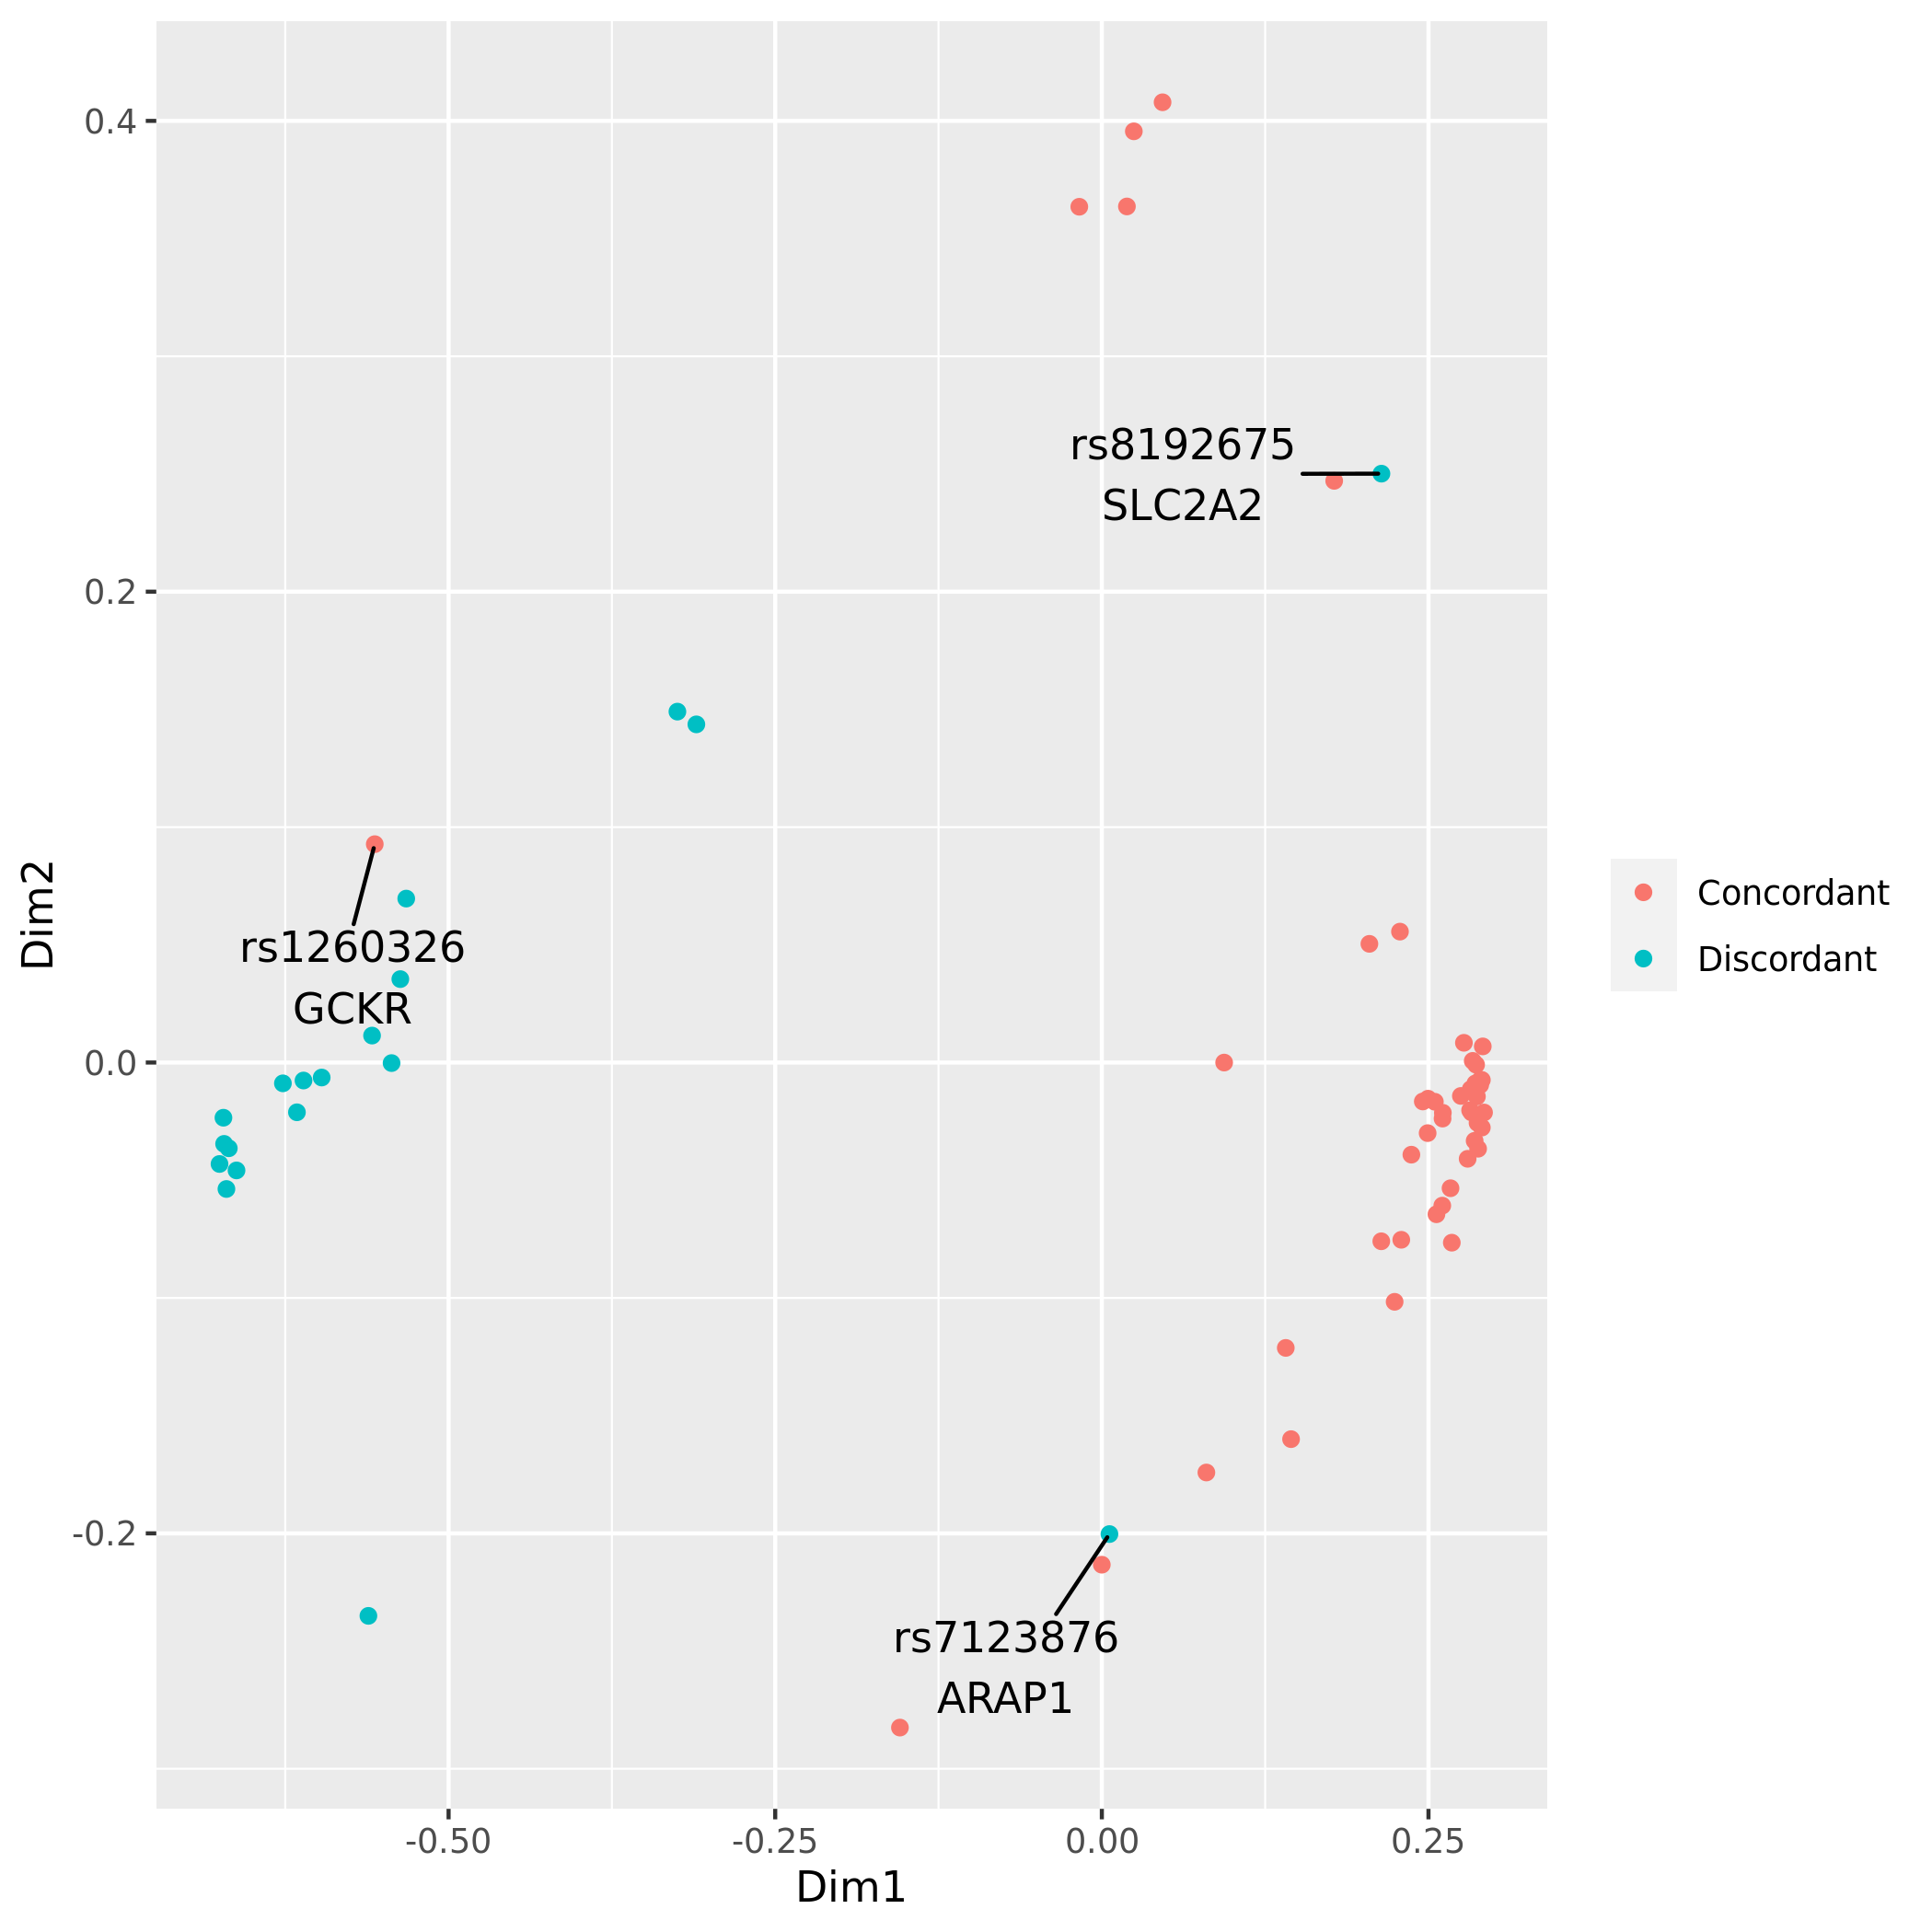
\includegraphics[width=6cm]{./plots/mds_phen.png}
\end{center}
\end{frame}

\begin{frame}[label={sec:org5b9df10}]{Heatmap of SNP effects on traits selected}
\begin{center}
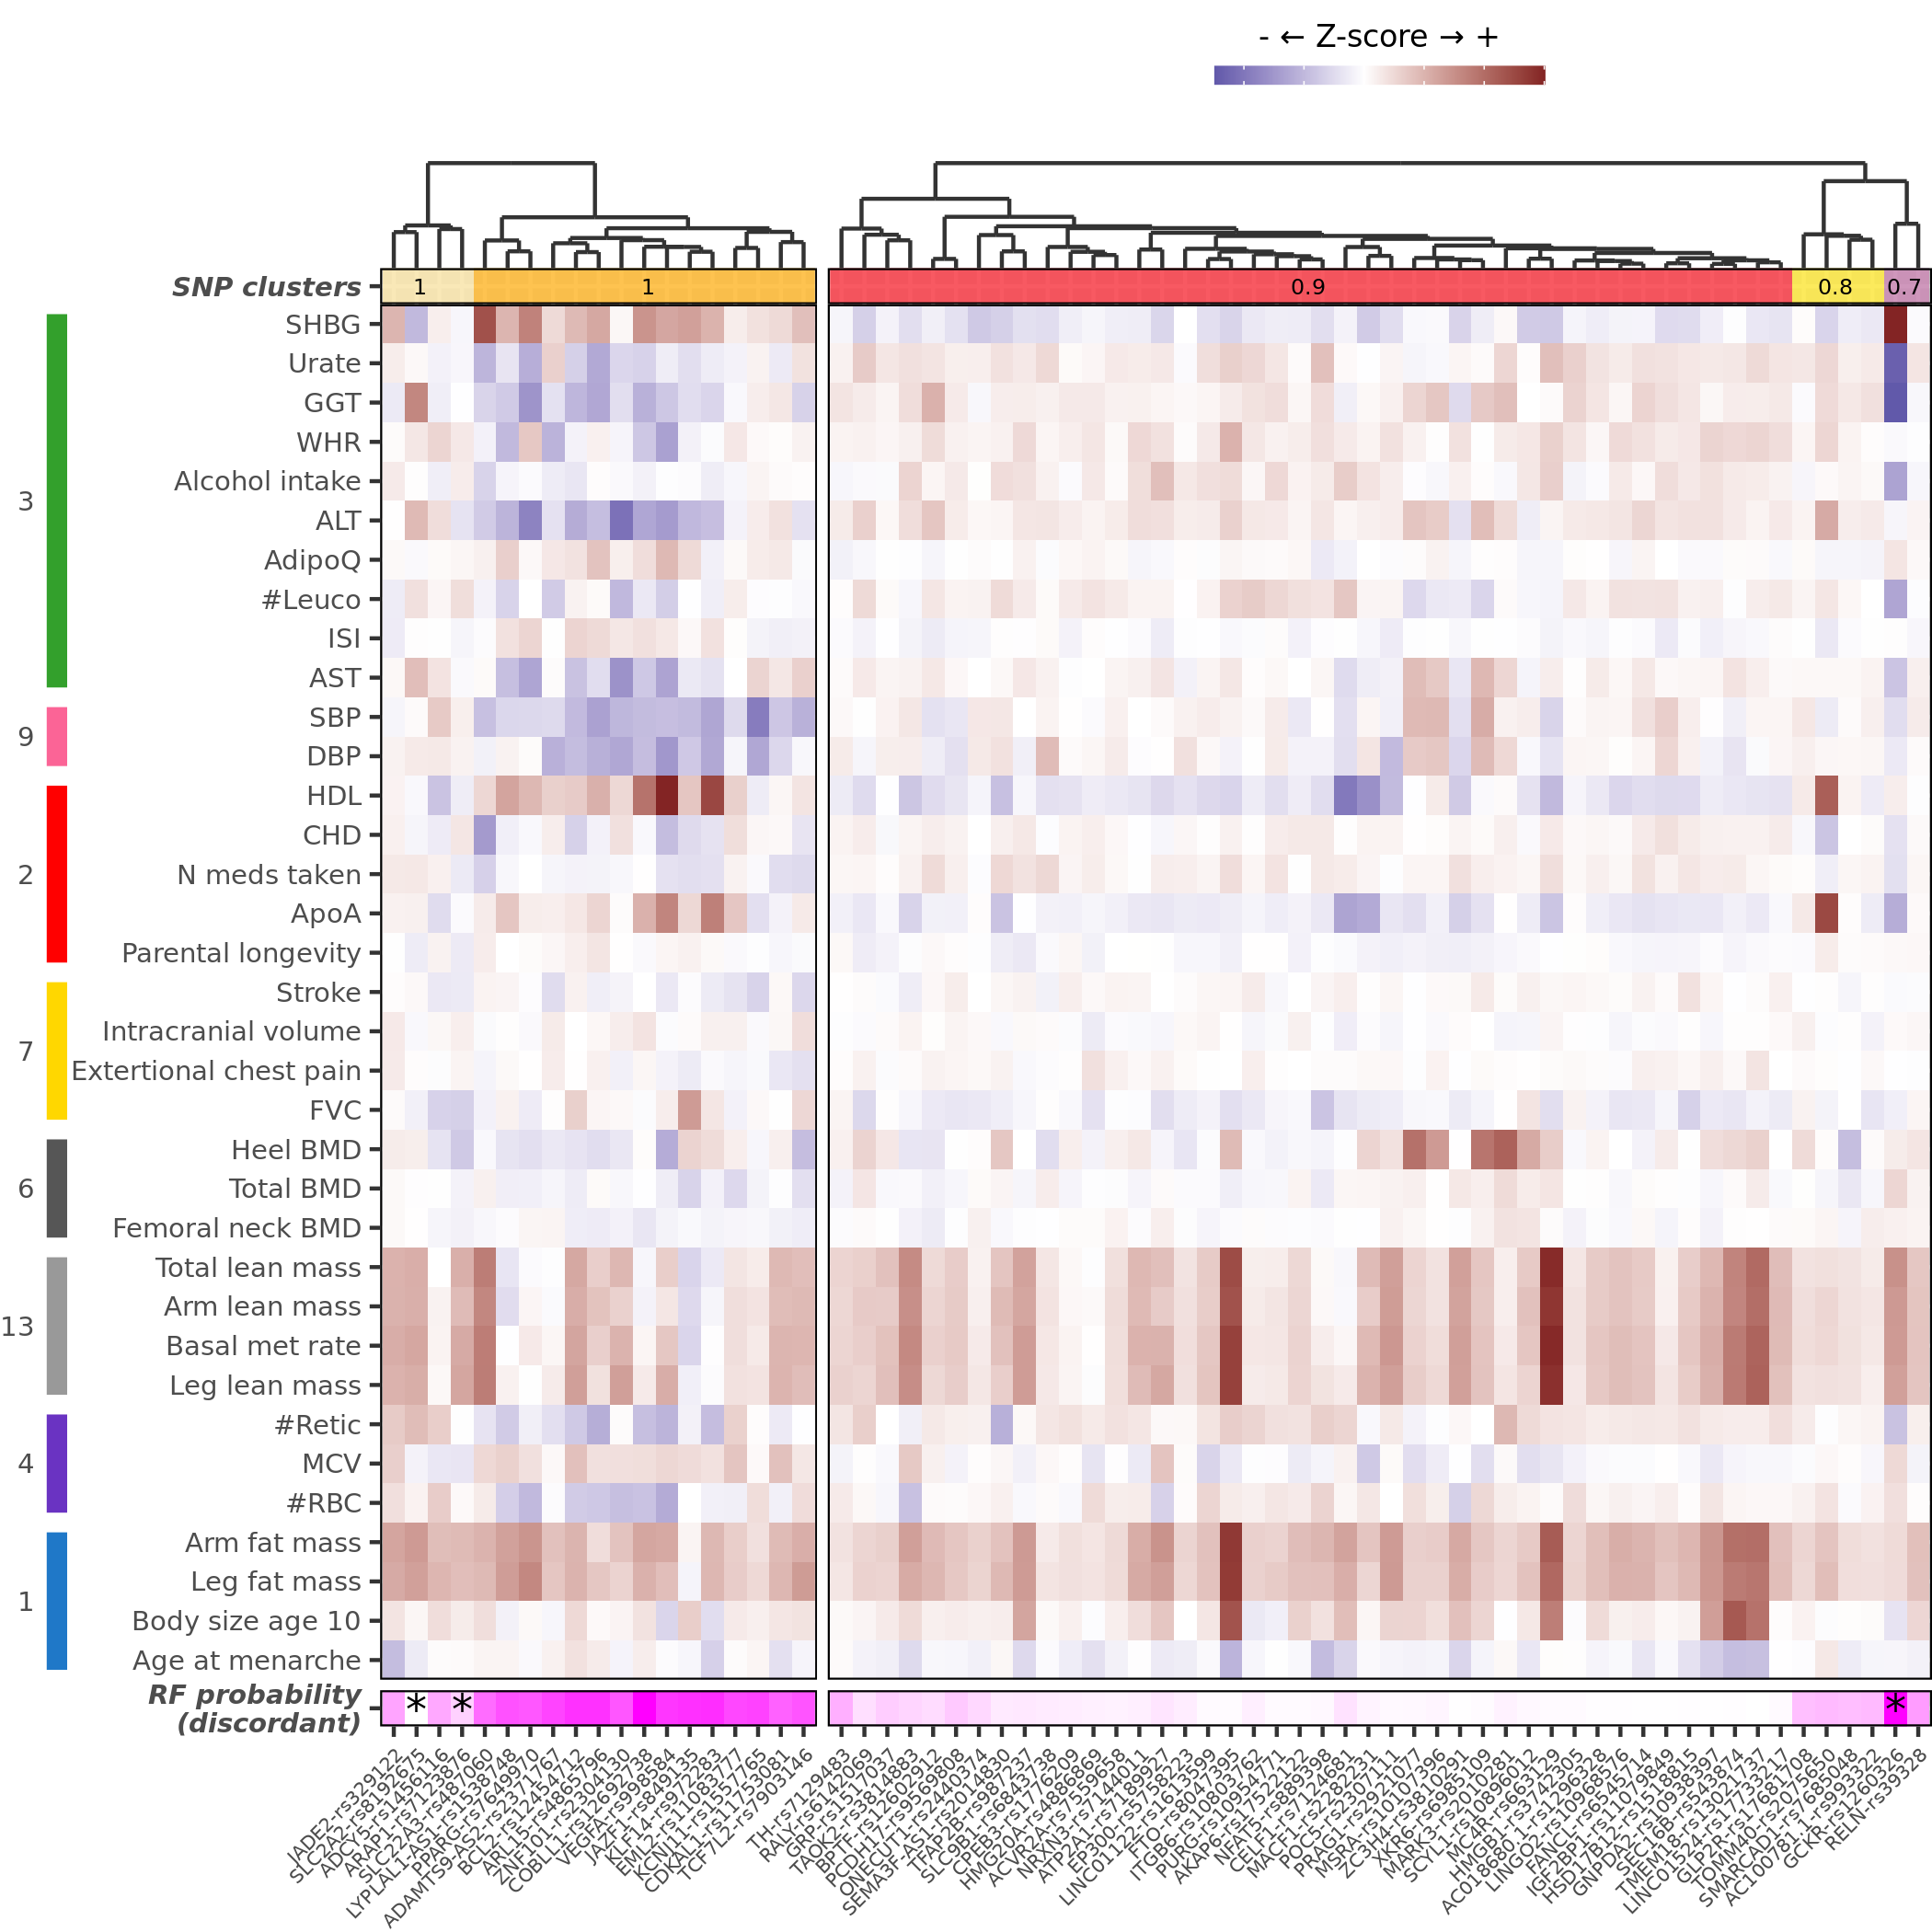
\includegraphics[width=7cm]{./plots/phen_hm.png}
\end{center}
\end{frame}

\begin{frame}[label={sec:org62f9d73}]{External validation - BioVU PheWAS}
\begin{itemize}
\item Associations with diagnostic codes (FDR 5\%)
\end{itemize}
\begin{center}
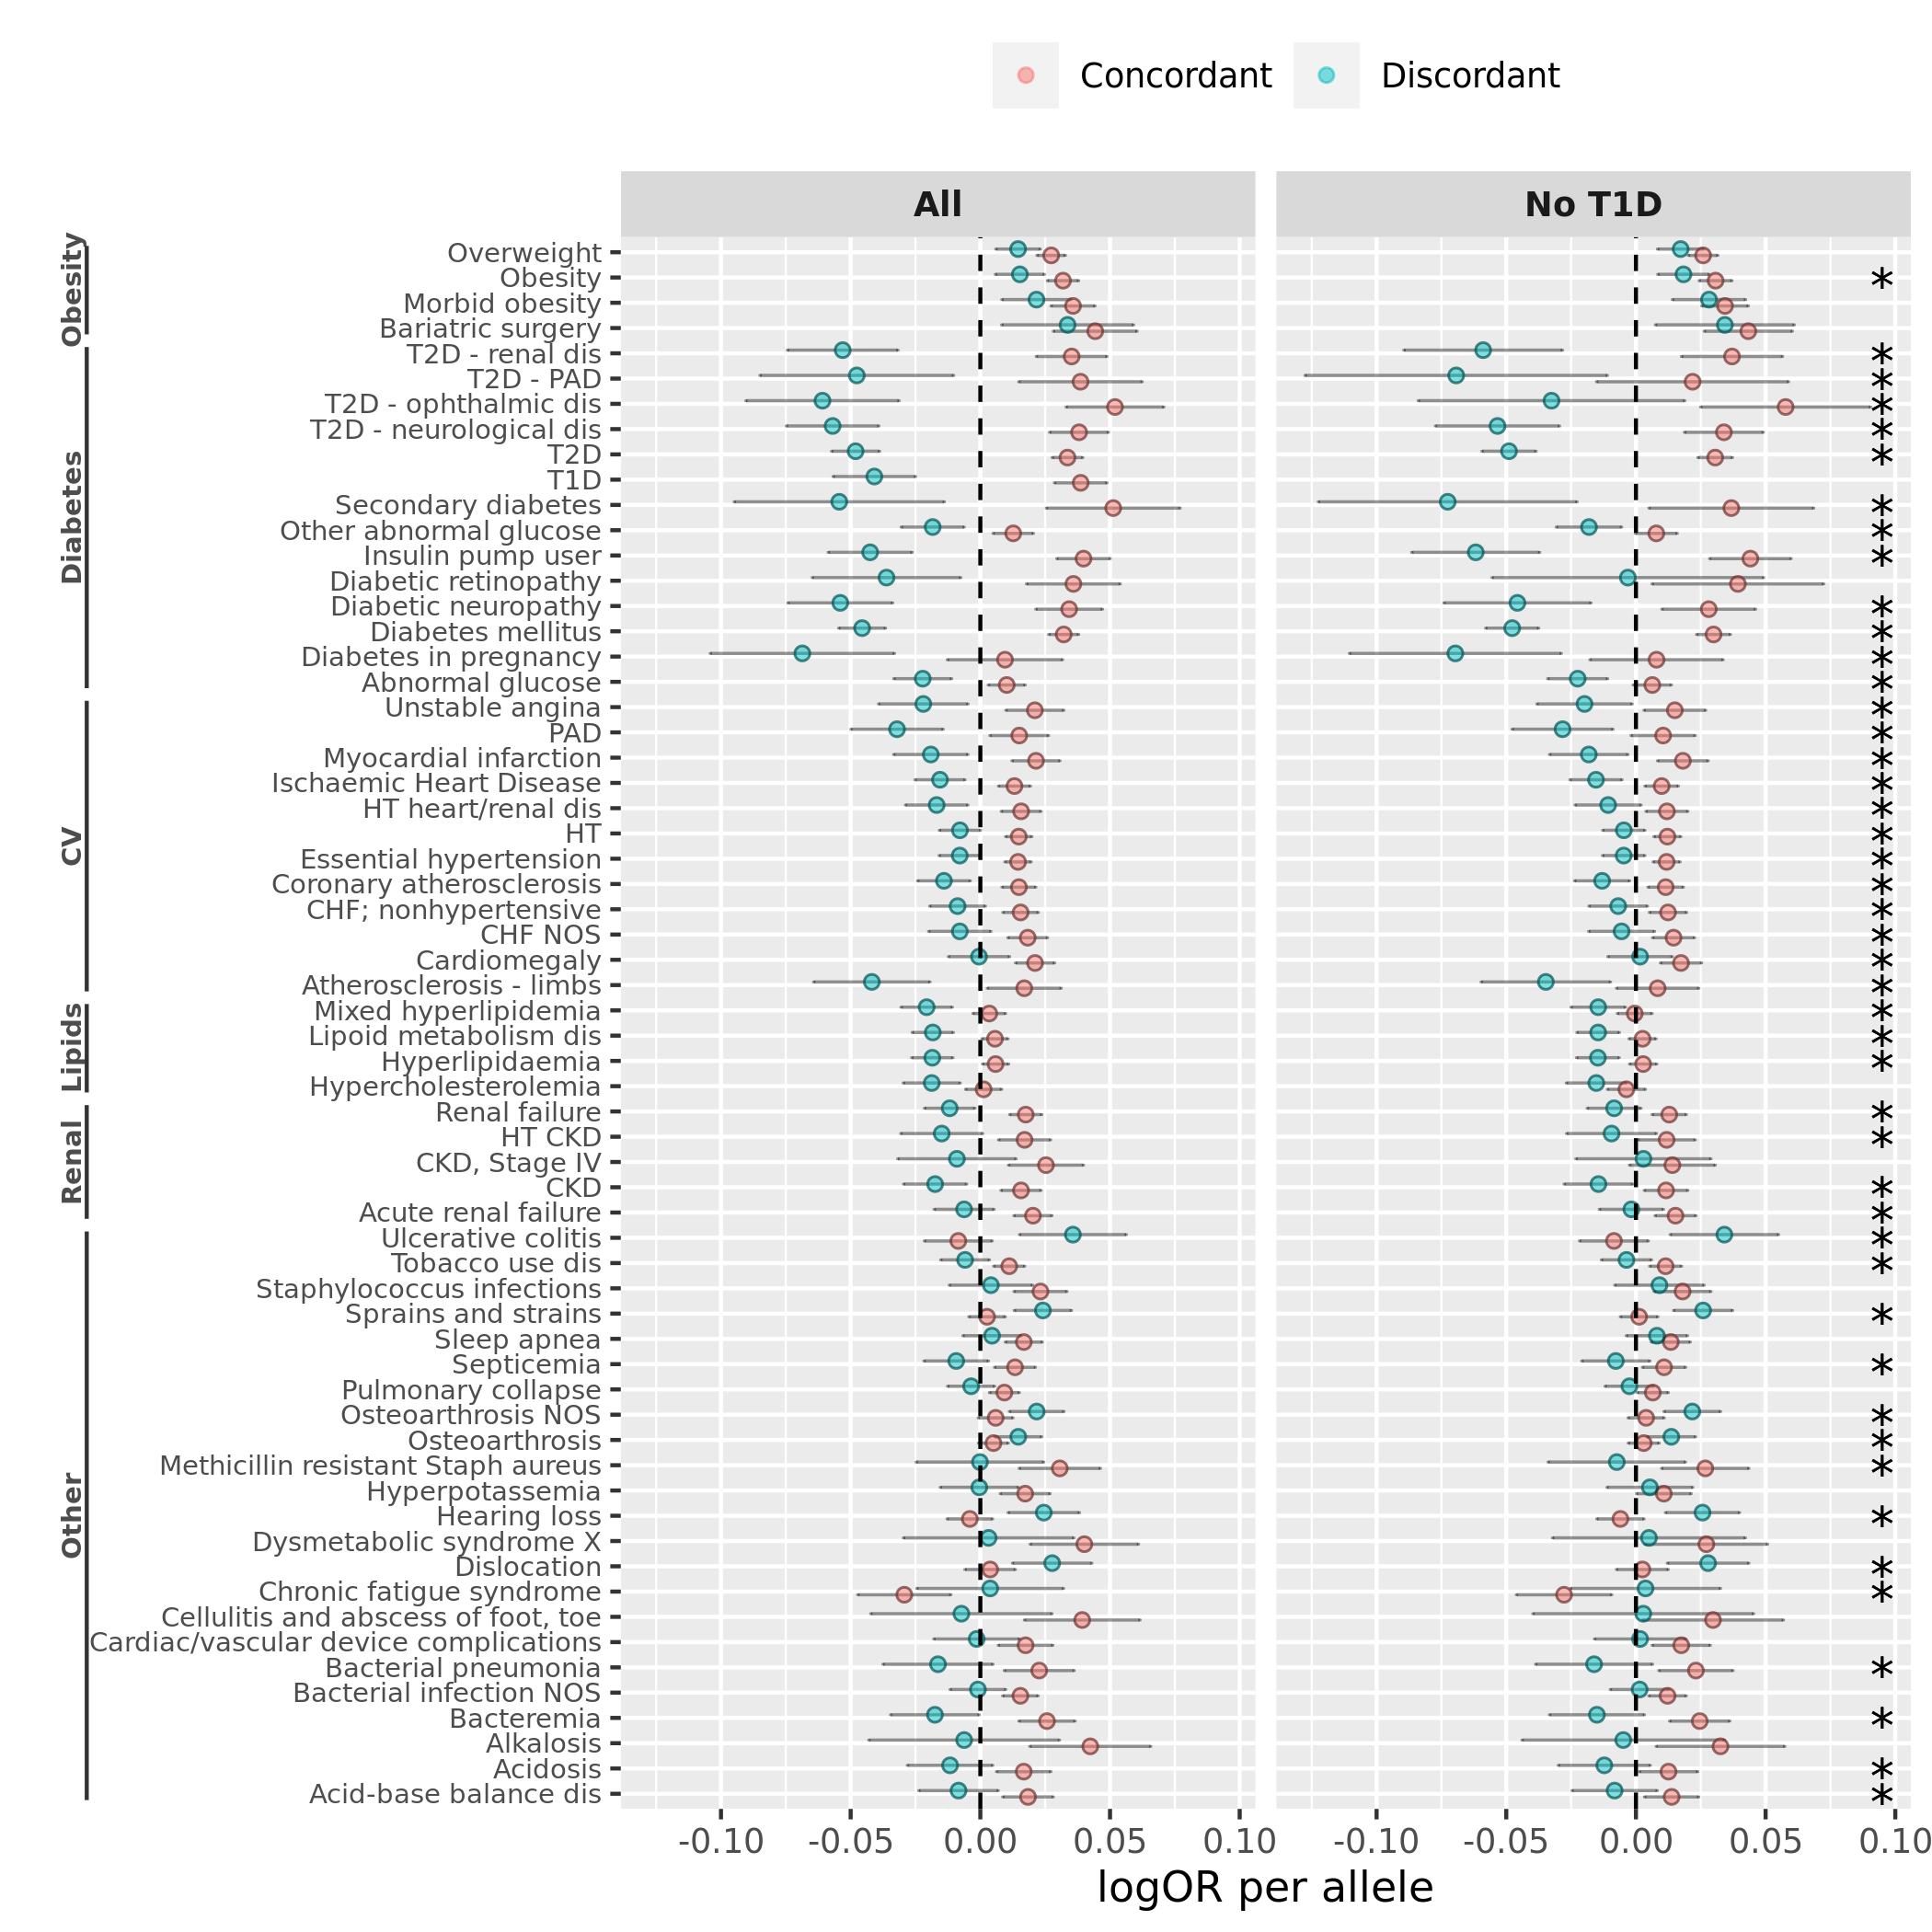
\includegraphics[width=7cm]{./plots/biovu_pw.png}
\end{center}
\end{frame}

\begin{frame}[label={sec:org056936b}]{External validation - BioVU LabWAS}
\begin{itemize}
\item Associations with median values of laboratory measurements per individual in BioVU (FDR 5\%)
\end{itemize}
\begin{center}
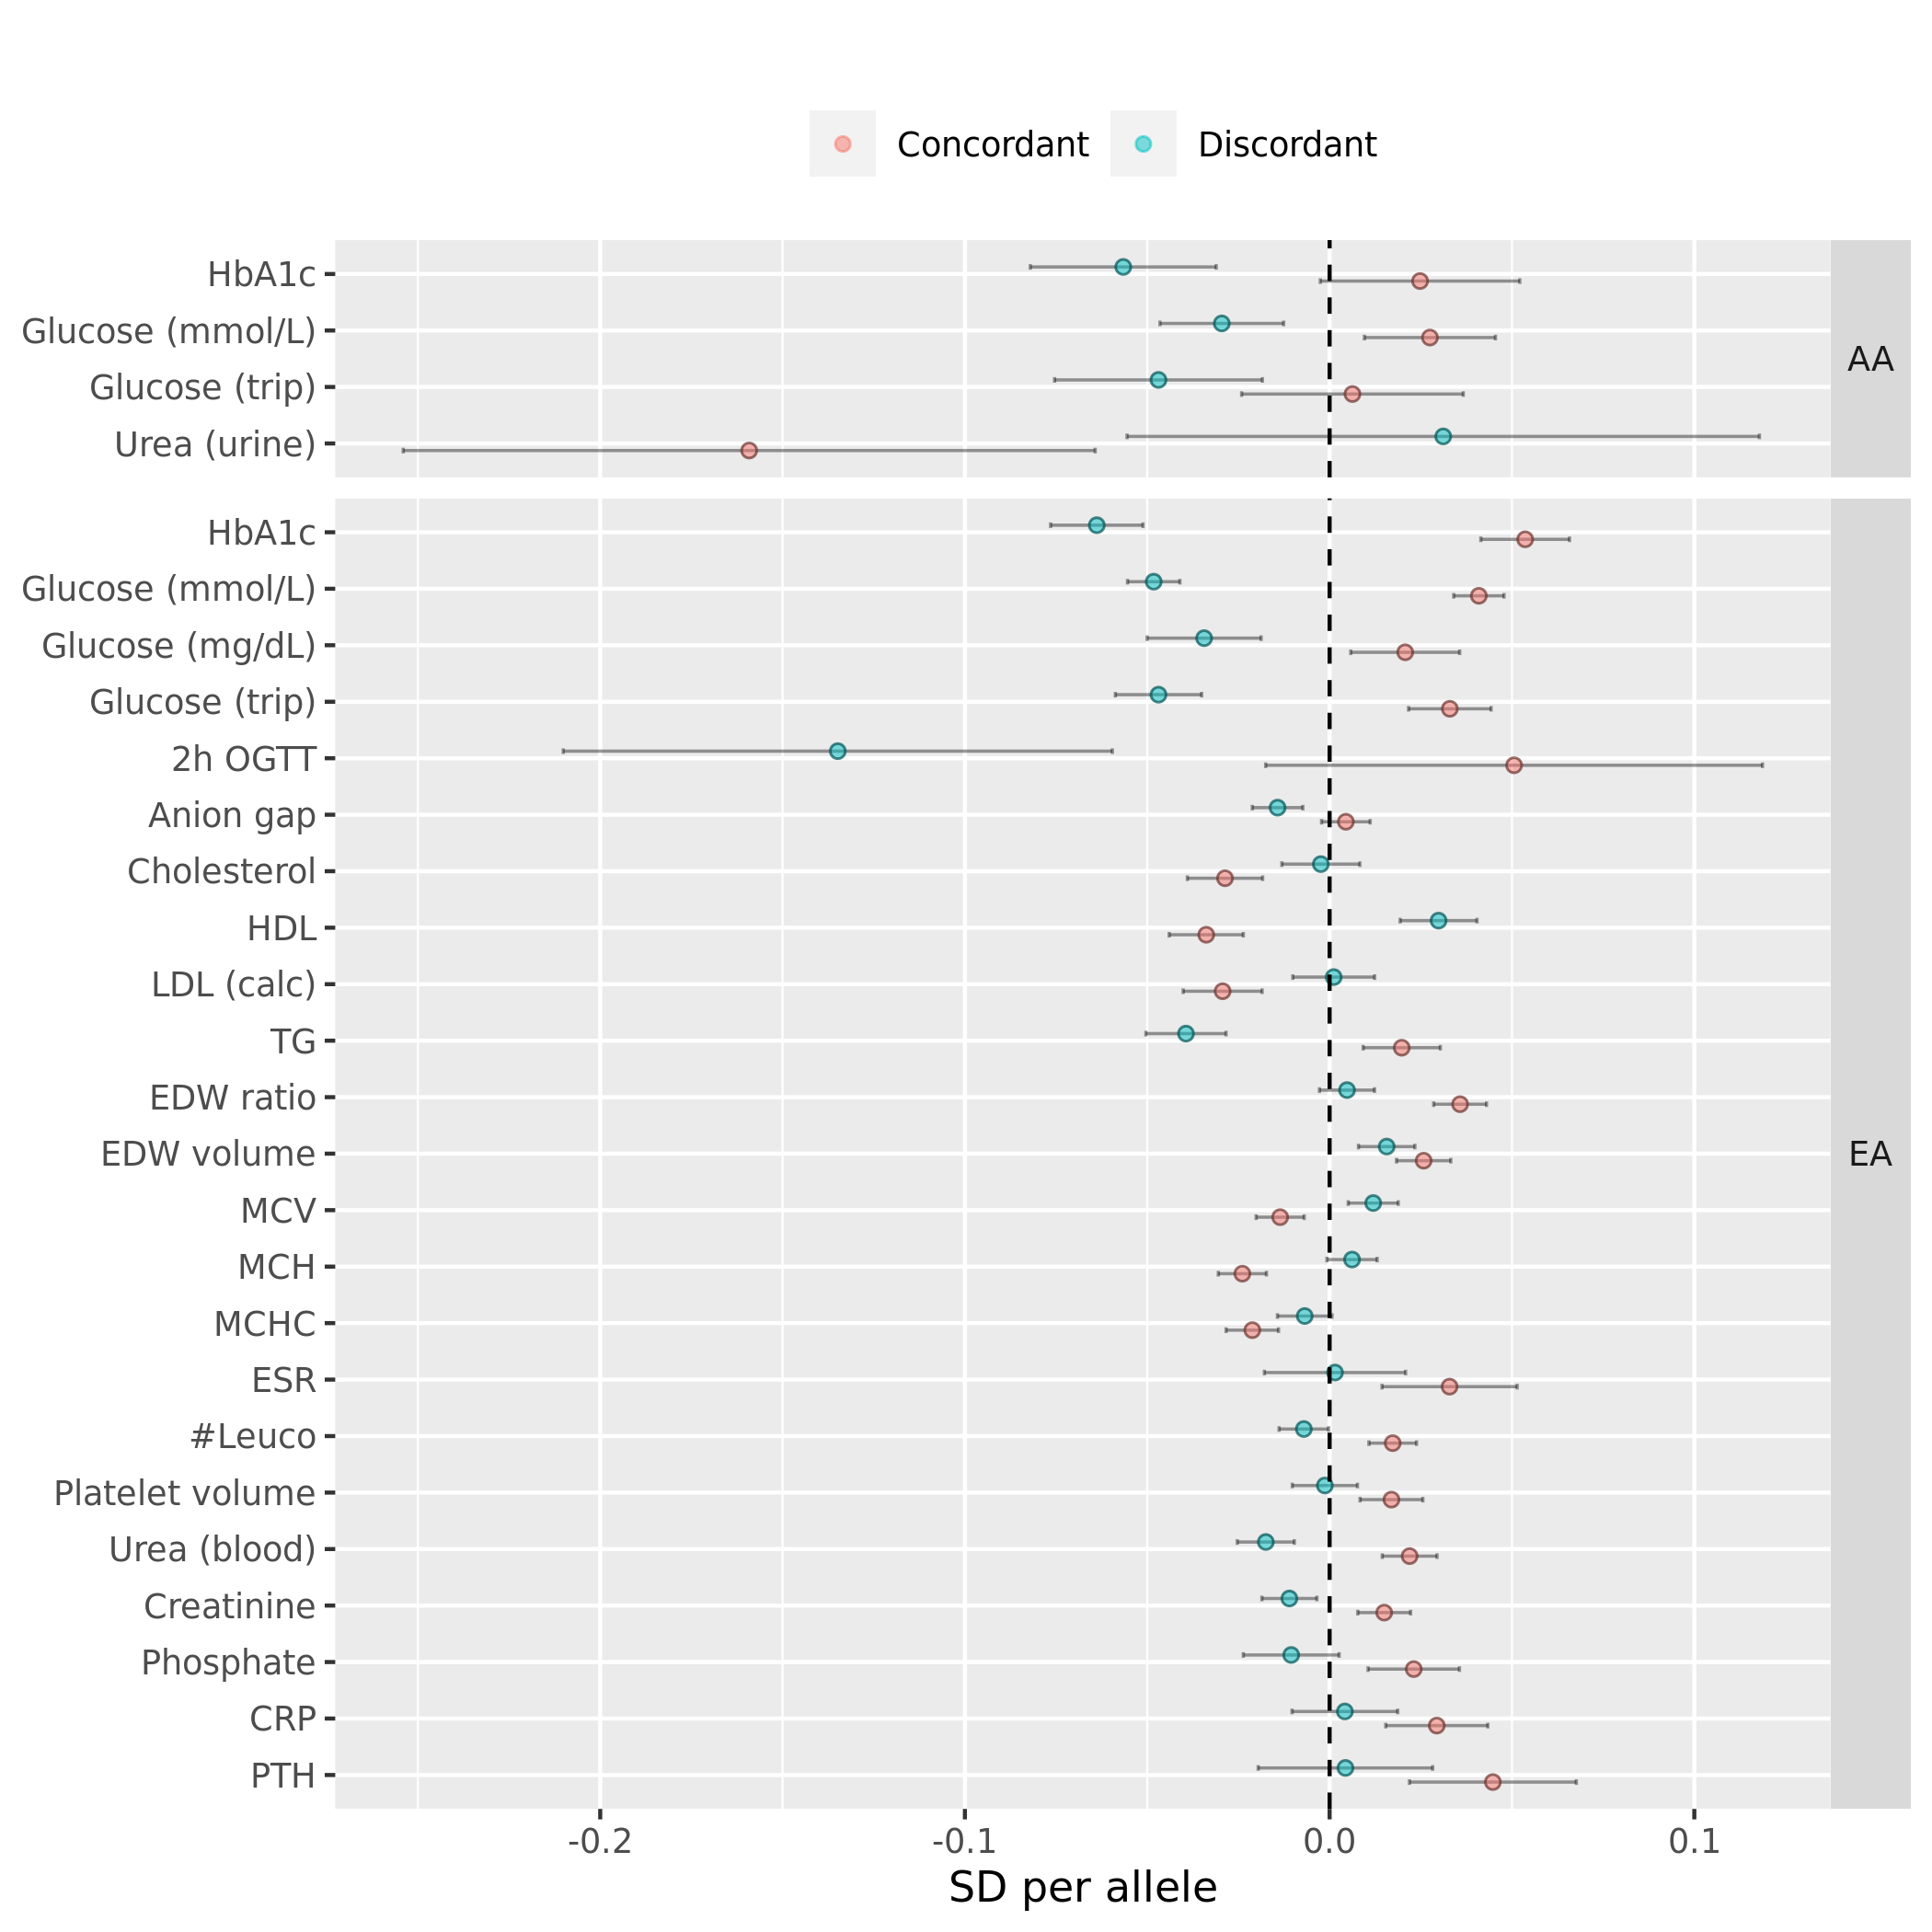
\includegraphics[width=6cm]{./plots/lw_biovu.png}
\end{center}
\end{frame}

\begin{frame}[label={sec:orgaa8bc50}]{Mortality in UK Biobank - Concordant vs Discordant SNPs}
\begin{center}
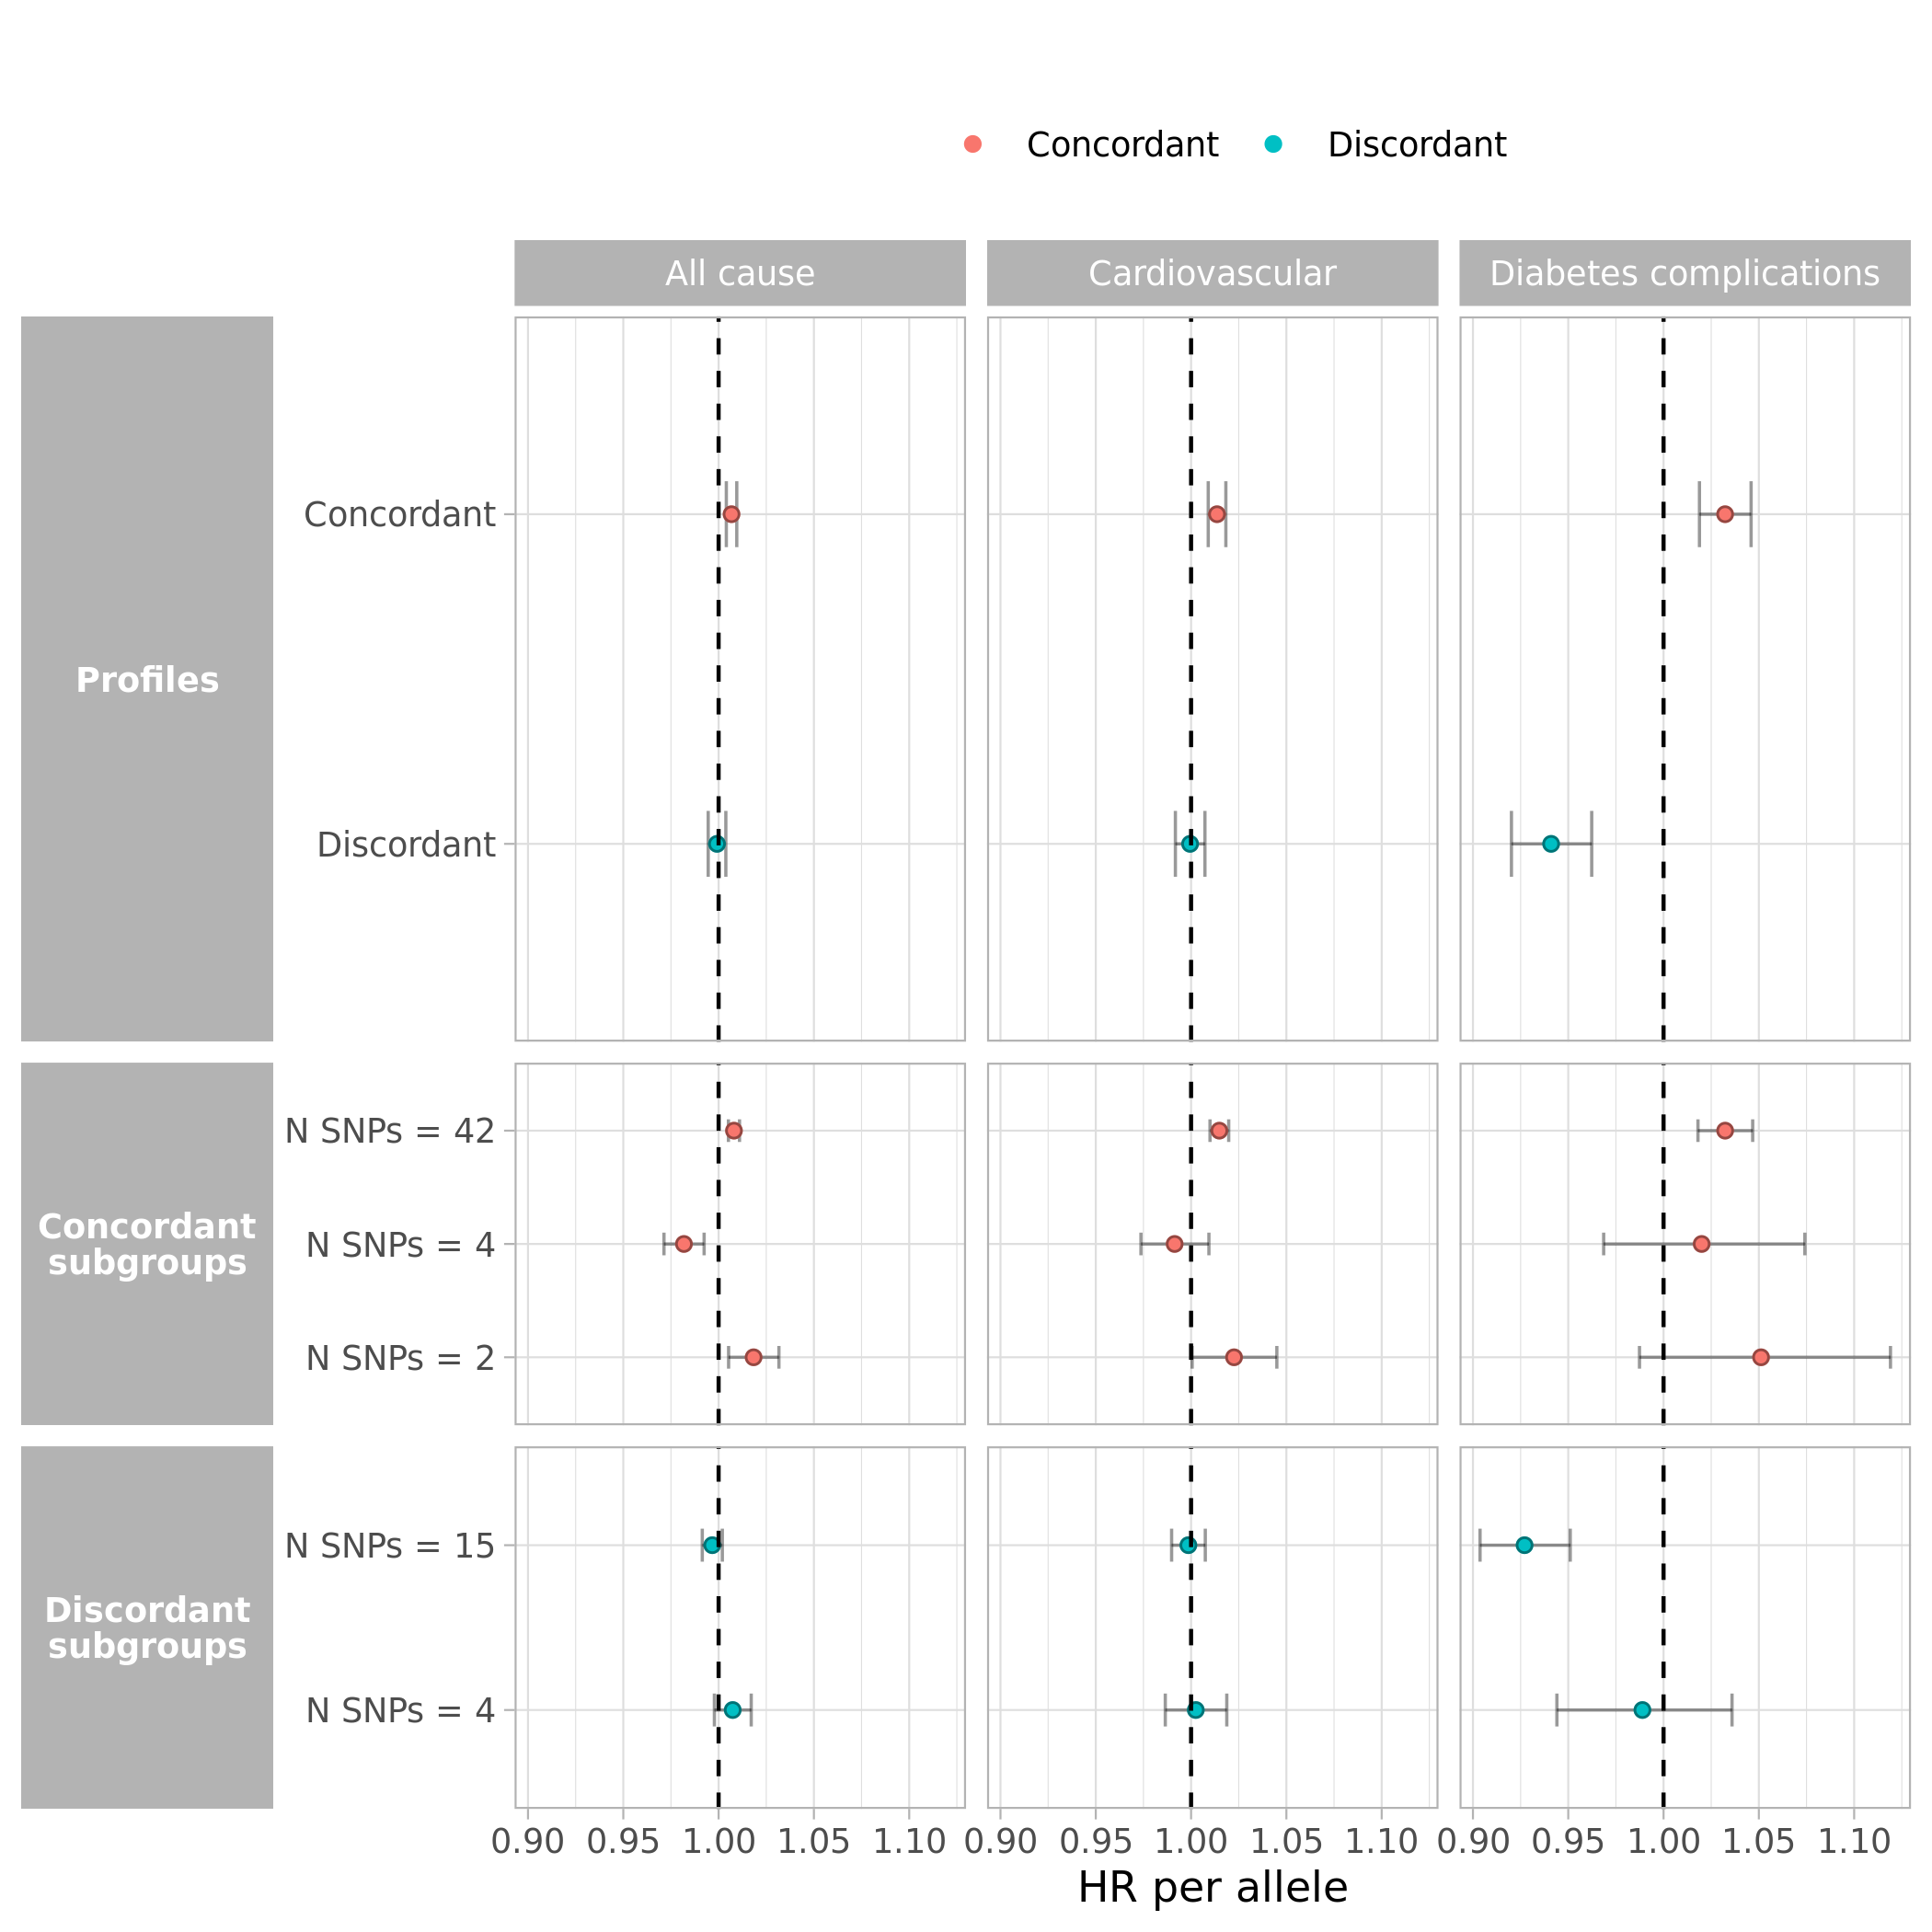
\includegraphics[width=6cm]{./plots/prs_surv.png}
\end{center}
\end{frame}

\begin{frame}[label={sec:org1437c0a}]{Mendelian Randomization}
\begin{center}
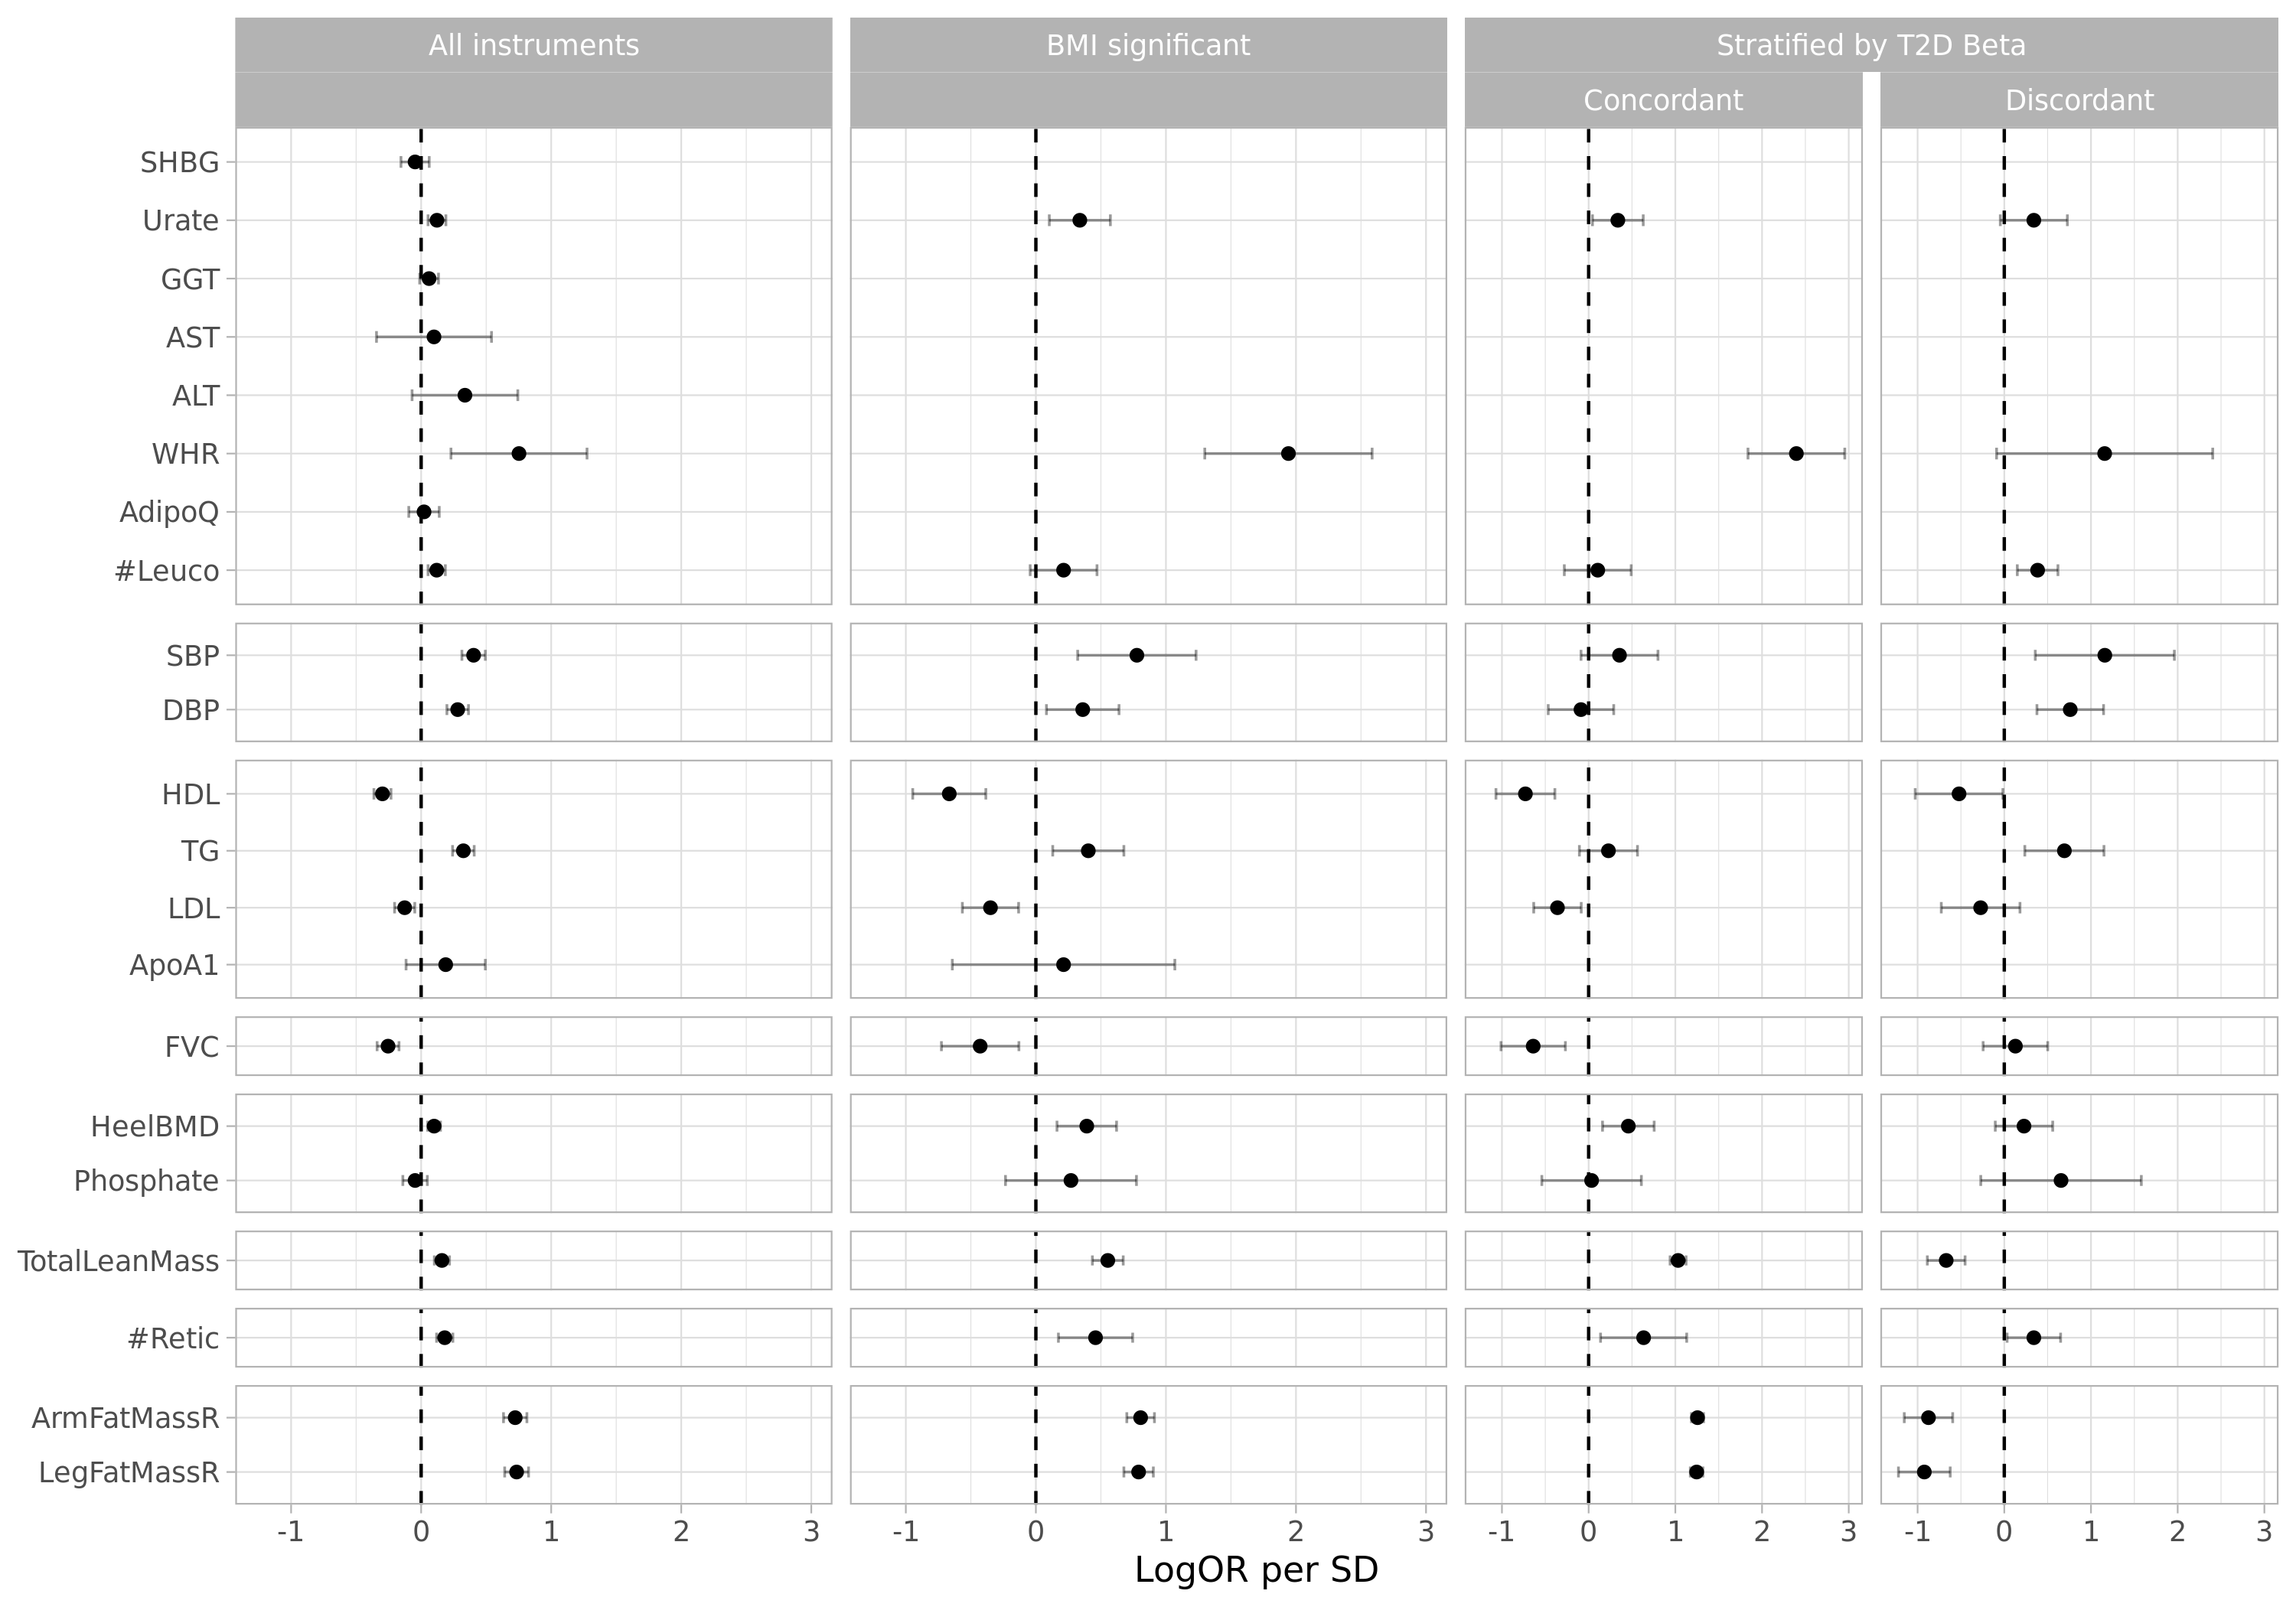
\includegraphics[width=.9\linewidth]{./plots/mr_res.png}
\end{center}
\end{frame}
\end{document}
